% Options for packages loaded elsewhere
\PassOptionsToPackage{unicode}{hyperref}
\PassOptionsToPackage{hyphens}{url}
%
\documentclass[
  openany]{book}
\usepackage{amsmath,amssymb}
\usepackage{lmodern}
\usepackage{ifxetex,ifluatex}
\ifnum 0\ifxetex 1\fi\ifluatex 1\fi=0 % if pdftex
  \usepackage[T1]{fontenc}
  \usepackage[utf8]{inputenc}
  \usepackage{textcomp} % provide euro and other symbols
\else % if luatex or xetex
  \usepackage{unicode-math}
  \defaultfontfeatures{Scale=MatchLowercase}
  \defaultfontfeatures[\rmfamily]{Ligatures=TeX,Scale=1}
\fi
% Use upquote if available, for straight quotes in verbatim environments
\IfFileExists{upquote.sty}{\usepackage{upquote}}{}
\IfFileExists{microtype.sty}{% use microtype if available
  \usepackage[]{microtype}
  \UseMicrotypeSet[protrusion]{basicmath} % disable protrusion for tt fonts
}{}
\makeatletter
\@ifundefined{KOMAClassName}{% if non-KOMA class
  \IfFileExists{parskip.sty}{%
    \usepackage{parskip}
  }{% else
    \setlength{\parindent}{0pt}
    \setlength{\parskip}{6pt plus 2pt minus 1pt}}
}{% if KOMA class
  \KOMAoptions{parskip=half}}
\makeatother
\usepackage{xcolor}
\IfFileExists{xurl.sty}{\usepackage{xurl}}{} % add URL line breaks if available
\IfFileExists{bookmark.sty}{\usepackage{bookmark}}{\usepackage{hyperref}}
\hypersetup{
  pdftitle={Addressing Neglect in the Private Rental Market},
  pdfauthor={Sarah Johnson},
  hidelinks,
  pdfcreator={LaTeX via pandoc}}
\urlstyle{same} % disable monospaced font for URLs
\usepackage{color}
\usepackage{fancyvrb}
\newcommand{\VerbBar}{|}
\newcommand{\VERB}{\Verb[commandchars=\\\{\}]}
\DefineVerbatimEnvironment{Highlighting}{Verbatim}{commandchars=\\\{\}}
% Add ',fontsize=\small' for more characters per line
\usepackage{framed}
\definecolor{shadecolor}{RGB}{248,248,248}
\newenvironment{Shaded}{\begin{snugshade}}{\end{snugshade}}
\newcommand{\AlertTok}[1]{\textcolor[rgb]{0.94,0.16,0.16}{#1}}
\newcommand{\AnnotationTok}[1]{\textcolor[rgb]{0.56,0.35,0.01}{\textbf{\textit{#1}}}}
\newcommand{\AttributeTok}[1]{\textcolor[rgb]{0.77,0.63,0.00}{#1}}
\newcommand{\BaseNTok}[1]{\textcolor[rgb]{0.00,0.00,0.81}{#1}}
\newcommand{\BuiltInTok}[1]{#1}
\newcommand{\CharTok}[1]{\textcolor[rgb]{0.31,0.60,0.02}{#1}}
\newcommand{\CommentTok}[1]{\textcolor[rgb]{0.56,0.35,0.01}{\textit{#1}}}
\newcommand{\CommentVarTok}[1]{\textcolor[rgb]{0.56,0.35,0.01}{\textbf{\textit{#1}}}}
\newcommand{\ConstantTok}[1]{\textcolor[rgb]{0.00,0.00,0.00}{#1}}
\newcommand{\ControlFlowTok}[1]{\textcolor[rgb]{0.13,0.29,0.53}{\textbf{#1}}}
\newcommand{\DataTypeTok}[1]{\textcolor[rgb]{0.13,0.29,0.53}{#1}}
\newcommand{\DecValTok}[1]{\textcolor[rgb]{0.00,0.00,0.81}{#1}}
\newcommand{\DocumentationTok}[1]{\textcolor[rgb]{0.56,0.35,0.01}{\textbf{\textit{#1}}}}
\newcommand{\ErrorTok}[1]{\textcolor[rgb]{0.64,0.00,0.00}{\textbf{#1}}}
\newcommand{\ExtensionTok}[1]{#1}
\newcommand{\FloatTok}[1]{\textcolor[rgb]{0.00,0.00,0.81}{#1}}
\newcommand{\FunctionTok}[1]{\textcolor[rgb]{0.00,0.00,0.00}{#1}}
\newcommand{\ImportTok}[1]{#1}
\newcommand{\InformationTok}[1]{\textcolor[rgb]{0.56,0.35,0.01}{\textbf{\textit{#1}}}}
\newcommand{\KeywordTok}[1]{\textcolor[rgb]{0.13,0.29,0.53}{\textbf{#1}}}
\newcommand{\NormalTok}[1]{#1}
\newcommand{\OperatorTok}[1]{\textcolor[rgb]{0.81,0.36,0.00}{\textbf{#1}}}
\newcommand{\OtherTok}[1]{\textcolor[rgb]{0.56,0.35,0.01}{#1}}
\newcommand{\PreprocessorTok}[1]{\textcolor[rgb]{0.56,0.35,0.01}{\textit{#1}}}
\newcommand{\RegionMarkerTok}[1]{#1}
\newcommand{\SpecialCharTok}[1]{\textcolor[rgb]{0.00,0.00,0.00}{#1}}
\newcommand{\SpecialStringTok}[1]{\textcolor[rgb]{0.31,0.60,0.02}{#1}}
\newcommand{\StringTok}[1]{\textcolor[rgb]{0.31,0.60,0.02}{#1}}
\newcommand{\VariableTok}[1]{\textcolor[rgb]{0.00,0.00,0.00}{#1}}
\newcommand{\VerbatimStringTok}[1]{\textcolor[rgb]{0.31,0.60,0.02}{#1}}
\newcommand{\WarningTok}[1]{\textcolor[rgb]{0.56,0.35,0.01}{\textbf{\textit{#1}}}}
\usepackage{longtable,booktabs,array}
\usepackage{calc} % for calculating minipage widths
% Correct order of tables after \paragraph or \subparagraph
\usepackage{etoolbox}
\makeatletter
\patchcmd\longtable{\par}{\if@noskipsec\mbox{}\fi\par}{}{}
\makeatother
% Allow footnotes in longtable head/foot
\IfFileExists{footnotehyper.sty}{\usepackage{footnotehyper}}{\usepackage{footnote}}
\makesavenoteenv{longtable}
\usepackage{graphicx}
\makeatletter
\def\maxwidth{\ifdim\Gin@nat@width>\linewidth\linewidth\else\Gin@nat@width\fi}
\def\maxheight{\ifdim\Gin@nat@height>\textheight\textheight\else\Gin@nat@height\fi}
\makeatother
% Scale images if necessary, so that they will not overflow the page
% margins by default, and it is still possible to overwrite the defaults
% using explicit options in \includegraphics[width, height, ...]{}
\setkeys{Gin}{width=\maxwidth,height=\maxheight,keepaspectratio}
% Set default figure placement to htbp
\makeatletter
\def\fps@figure{htbp}
\makeatother
\setlength{\emergencystretch}{3em} % prevent overfull lines
\providecommand{\tightlist}{%
  \setlength{\itemsep}{0pt}\setlength{\parskip}{0pt}}
\setcounter{secnumdepth}{5}
\usepackage{booktabs}
\usepackage{booktabs}
\usepackage{longtable}
\usepackage{array}
\usepackage{multirow}
\usepackage{wrapfig}
\usepackage{float}
\usepackage{colortbl}
\usepackage{pdflscape}
\usepackage{tabu}
\usepackage{threeparttable}
\usepackage{threeparttablex}
\usepackage[normalem]{ulem}
\usepackage{makecell}
\usepackage{xcolor}
\ifluatex
  \usepackage{selnolig}  % disable illegal ligatures
\fi
\newlength{\cslhangindent}
\setlength{\cslhangindent}{1.5em}
\newlength{\csllabelwidth}
\setlength{\csllabelwidth}{3em}
\newenvironment{CSLReferences}[2] % #1 hanging-ident, #2 entry spacing
 {% don't indent paragraphs
  \setlength{\parindent}{0pt}
  % turn on hanging indent if param 1 is 1
  \ifodd #1 \everypar{\setlength{\hangindent}{\cslhangindent}}\ignorespaces\fi
  % set entry spacing
  \ifnum #2 > 0
  \setlength{\parskip}{#2\baselineskip}
  \fi
 }%
 {}
\usepackage{calc}
\newcommand{\CSLBlock}[1]{#1\hfill\break}
\newcommand{\CSLLeftMargin}[1]{\parbox[t]{\csllabelwidth}{#1}}
\newcommand{\CSLRightInline}[1]{\parbox[t]{\linewidth - \csllabelwidth}{#1}\break}
\newcommand{\CSLIndent}[1]{\hspace{\cslhangindent}#1}

\title{Addressing Neglect in the Private Rental Market}
\author{Sarah Johnson}
\date{2021-08-05}

\begin{document}
\maketitle

{
\setcounter{tocdepth}{1}
\tableofcontents
}
\hypertarget{about-the-author}{%
\chapter*{About the Author}\label{about-the-author}}
\addcontentsline{toc}{chapter}{About the Author}

Sarah Johnson is completing her master's in City and Regional Planning from the University of Memphis (expected graduation August 2021).

\hypertarget{intro}{%
\chapter{Introduction}\label{intro}}

In recent years, housing discourse has been dominated by high rates of cost burdenship and the need for affordable rental housing. Less discussed is the need for improved housing quality, particularly in the private rental sector. Housing quality and health have been extensively linked by the public health field, yet tenants who wish to improve their housing quality risk possible retaliation, including increased rents and eviction. Current regulations assume that tenants will take action to report substandard housing, ignoring the risk to a tenant's housing stability. As such, substandard housing is heavily under-reported to code enforcement, often not on their radar till the housing structure is in major disrepair. At this point, the home may be condemned, deemed blighted and demolished, further decreasing the supply of low-rent housing.

This paper seeks to understand the extent of this problem in Memphis. The city has a large percentage of low-income renters, an aging housing stock, a high eviction rate, and high rates of asthma. Particular attention is given to code enforcement policies and data, and how the program has and has not changed over the past twenty years. I conclude with specific recommendations for how to improve code enforcement practices to target the needs of renters.

\hypertarget{housing-and-health}{%
\chapter{Housing and Health}\label{housing-and-health}}

\begin{quote}
Shelter is one of the three fundamental needs of human existence. No housing program can be sound unless the shelter it provides is healthful.

C.-E. A. Winslow, Dr.P.H., \emph{Chairman},\\
Allan A. Twichell, \emph{Technical Secretary},\\
\emph{Committee on the Hygiene of Housing (Mar., 1938)}
\end{quote}

\hypertarget{history}{%
\section{History}\label{history}}

The link between health and housing is long and well established.

On January 20, 1852, Dr.~John H. Griscom stood before an audience and spoke on the importance of clean air, a topic he believed ``was not so much studied as it ought to be.'' The lecture was summarized on the front page of the New-York Daily Times the next day, concluding with Dr.~Griscom's statement that ``ventilation in houses should be attended to as one of the best means of preserving health.''\footnote{\protect\hyperlink{ref-lectures1852}{{``Lectures for the People; the Importance of Proper Vetilation.''} \emph{The New York Times}, January 21, 1852, \url{https://www.nytimes.com/1852/01/21/archives/lectures-for-the-people-the-importance-of-proper-vetilation-a.html}}.}

The idea must have caught on---two and a half years later, an article describing the poor conditions of a building in Buffalo declared, ``we intended to speak on the ventilation, but we are sick of the subject.''\footnote{\protect\hyperlink{ref-thebuff1854}{{``The Buffalo Poor-House: Horrible Particulars of Its Condition.''} \emph{The New York Times}, July 24, 1854, \url{https://www.nytimes.com/1854/07/24/archives/the-buffalo-poorhousehorrible-particulars-of-its-condition.html}}.} The home in question had recently been investigated by the local Board of Health based on rumors of high mortality among residents. The authors, after listing the horrid living conditions, concluded on a positive note that they were thankful to ``have a Board of Health which we believe will do its duty\ldots to reform this great abuse.''

Over the next half century, large population influx into urban areas led to widespread development of tenement housing.\footnote{\protect\hyperlink{ref-soifer2014}{Steven Soifer et al., \emph{Community Economic Development in Social Work} (Columbia University Press, 2014), 7}.} These homes offered little in the way of space, sanitation, light, or fresh air, a fact made well-known by Jacob Riis's 1890 book \emph{How the Other Half Lives}. The conditions documented by Riis led New York City to adopt the first housing code in the United States.

Housing reformers continued to demand better living conditions into the 20th century. Catherine Bauer's landmark 1934 book \emph{Modern Housing} declared that for a home to be ``modern,'' it must allow for cross-ventilation and sunlight; adequate privacy, space, and sanitary facilities; adjacent play space for children; and ``finally it will be available at a price which citizens of average income or less can afford.''\footnote{\protect\hyperlink{ref-wurster2020}{Catherine Bauer Wurster and Barbara Penner, \emph{Modern Housing} (Minneapolis: University of Minnesota Press, 2020)} xv.} Modern housing was constructed for ``efficient use'' rather than ``quick profit,'' and planned to retain quality for the long term, in ``complete neighborhoods'' with parks, schools, and other community facilities.

Her thesis was based on studies of post-war European housing programs, whom Bauer declared had created an entirely new framework for producing shelter.\footnote{\protect\hyperlink{ref-radford1996}{Gail Radford, \emph{Modern Housing for America}, 1996, 76, \url{https://press.uchicago.edu/ucp/books/book/chicago/M/bo3636758.html}}.} Bauer advocated for housing to be treated as a public utility, with a goal of comprehensively planned, decent, stable housing for the working class.\footnote{\protect\hyperlink{ref-goetz2013}{Edward G. Goetz, \emph{New Deal Ruins: Race, Economic Justice, and Public Housing Policy} (Ithaca: Cornell University Press, 2013), 23}; \protect\hyperlink{ref-radford1996}{Radford, \emph{Modern Housing for America}, 183}.} Modern homes and neighborhoods were a means to an end, and could ``never deteriorate into a slum, or a `blighted area'.''\footnote{\protect\hyperlink{ref-wurster2020}{Wurster and Penner, \emph{Modern Housing}} xv.}

This countered the limited federal housing legislation at the time, such as a post-Depression policy enacted under Hoover that provided loans to corporations wholly focused on low income housing and slum reconstruction.\footnote{\protect\hyperlink{ref-emergenc1932}{{``Emergency Relief and Construction Act of 1932,''} July 21, 1932, \url{https://uslaw.link/citation/us-law/public/72/302}}.} A lack of private investment led FDR to alter the program a year later to a public works initiative which directly funded construction of low cost housing and slum clearance projects.\footnote{\protect\hyperlink{ref-national1933}{{``National Industrial Recovery Act of 1933,''} June 16, 1933}; \protect\hyperlink{ref-goetz2013}{Goetz, \emph{New Deal Ruins}, 26}.}

Bauer was later a primary author on the National Housing Act of 1937, which officially established public housing in America and called for ``the elimination of unsafe and insanitary housing conditions'' and remedy ``the acute shortage of decent, safe, and sanitary dwellings for families of low-income, in rural or urban communities.''\footnote{\protect\hyperlink{ref-national1937}{{``National Housing Act of 1937,''} September 1, 1937}; \protect\hyperlink{ref-mccarty2019}{Maggie McCarty, Libby Perl, and Katie Jones, {``Overview of Federal Housing Assistance Programs and Policy,''} March 27, 2019}.}

However, the Act was a compromise. Limits were placed on construction costs and tenant incomes, and an ``equivalent elimination'' clause required one unit of substandard housing be taken down for every unit of public housing built. This ensured the bulk of public housing projects would be in previous slum areas, and was meant to prevent public housing from competing with the private market.\footnote{\protect\hyperlink{ref-goetz2013}{Goetz, \emph{New Deal Ruins}, 27--28}; \protect\hyperlink{ref-radford1996}{Radford, \emph{Modern Housing for America}, 188--89}.}\footnote{According to the bill's co-sponsor, Senator Wagner, ``the most important consideration is, that public housing projects should not be brought into competition with private industry\ldots{} To reach those who are really entitled to public assistance, and to get into the field where private enterprise cannot operate, is the objective of this bill.'' \protect\hyperlink{ref-federal1985}{J. Paul Mitchell, Lawrence M. Friedman, and Rutgers University, eds.} (\protect\hyperlink{ref-federal1985}{\emph{Federal Housing Policy and Programs: Past and Present} (New Brunswick, N.J: Center for Urban Policy Research, Rutgers University, 1985)}).

  The organizations that mobilized against the bill were the U.S. Chamber of Commerce, National Association of Real Estate Boards, the U.S. League of Building and Loans, and the National Retail Lumber Dealers Association (\protect\hyperlink{ref-radford1996}{Radford, \emph{Modern Housing for America}, 188}).}

\hypertarget{healthy-homes}{%
\section{Healthy Homes}\label{healthy-homes}}

The 1937 Act led to the creation of the \emph{Basic Principles of Healthful Housing}, published in the American Journal of Public Health. The manual outlined 30 principles ``believed to be fundamental minima required for the promotion of physical, mental, and social health,'' whether the housing be high or low cost, urban or rural.\footnote{\protect\hyperlink{ref-apha1938}{APHA, {``Basic Principles of Healthful Housing,''} \emph{American Journal of Public Health and the Nations Health} 28, no. 3 (March 1938): 351--72, doi:\href{https://doi.org/10.2105/AJPH.28.3.351}{10.2105/AJPH.28.3.351}}.} The fundamental needs were originally divided into four categories: physiological needs (e.g.~protection from elements), psychological needs (e.g.~adequate privacy), protection against contagion (e.g.~safe water supply), and protection against accidents (e.g.~fire prevention).

Six decades after \emph{Healthful Housing} was published, the manual found renewed relevance in 1999. Recognizing that ``health, home construction, and home maintenance are inseparable because of their overlapping goals,'' HUD and CDC joined together to launch the Healthy Homes Initiative.\footnote{\protect\hyperlink{ref-cdc2006}{CDC and HUD, {``Healthy Housing Reference Manual''} (Atlanta, 2006), 31, 34, \url{https://www.cdc.gov/nceh/publications/books/housing/housing.htm}}.} Many of the basic principles originally laid out in the 1938 manual were used to create the Healthy Home Rating System (HHRS)

The below table lists all 29 hazards of the modern HHRS, along with a short description and which populations are most vulnerable to the specific hazard (adopted from \protect\hyperlink{ref-HHRSlst}{HUD}\footnote{\protect\hyperlink{ref-HHRSlst}{{``The Effect of the Defect: Housing Hazards Identified in the Healthy Home Rating System''} n.d., \url{https://www.hud.gov/sites/documents/hhrschart.pdf}}.} ).

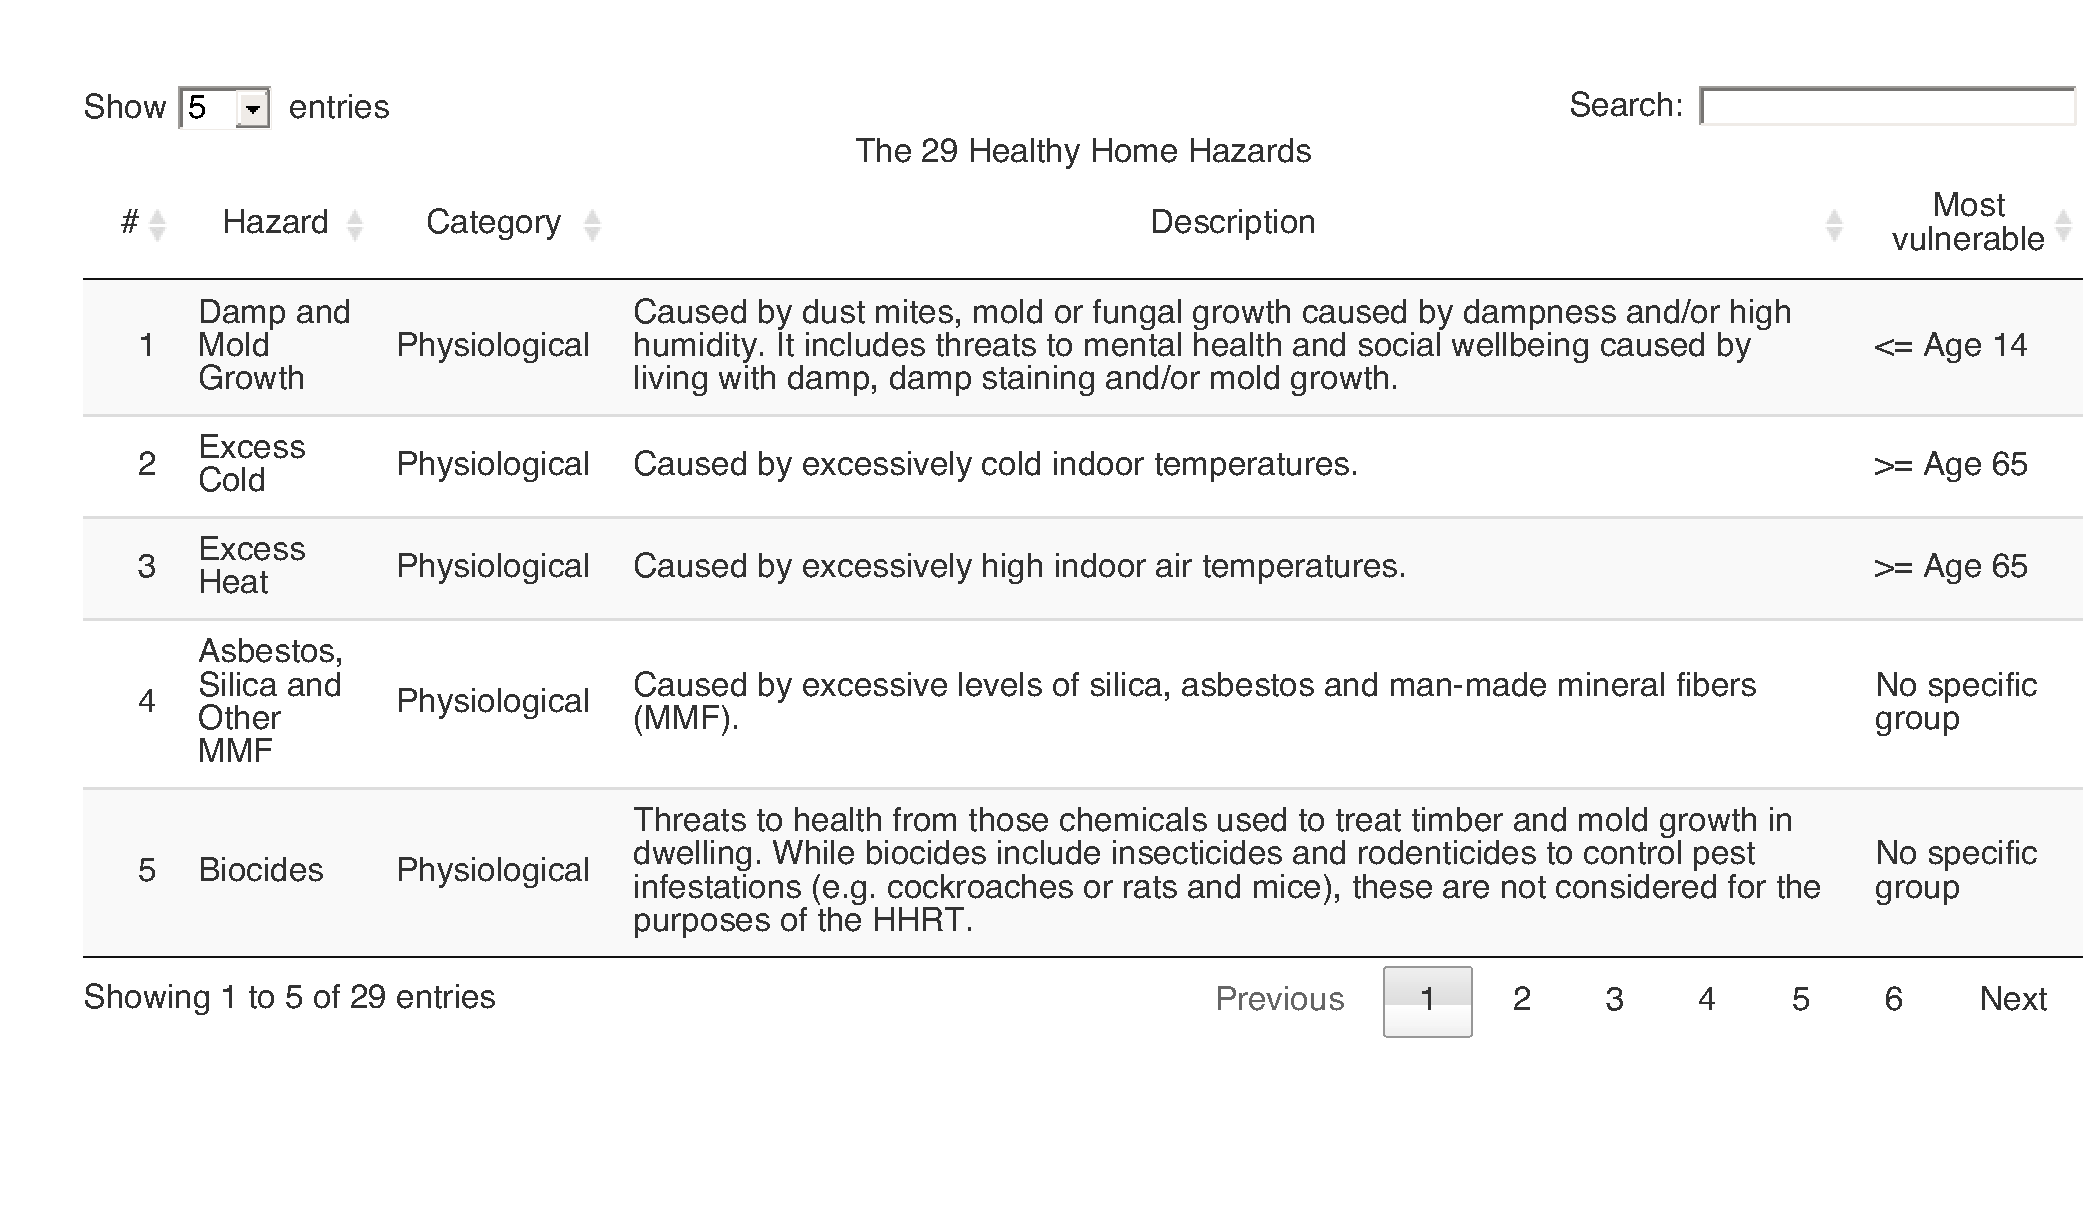
\includegraphics{MA-capstone_files/figure-latex/HHRStbl-1.pdf}

The HHRS provides a standardized way to identify and rate the risk of home health hazards. Once a hazard is identified, it is further rated according to severity and the effect it is having, or could have, on the occupants. The greater the risk or more serious the outcome, the higher the overall score. The system provides a way to compare risks associated with different types of hazards.

According to \protect\hyperlink{ref-HHRSover}{HUD},\footnote{\protect\hyperlink{ref-HHRSover}{{``Overview of the Healthy Home Rating System''} n.d., \url{https://www.hud.gov/sites/documents/OVERVIEW_HHRS.PDF}}.} this system lets local housing and health departments to know which hazards are most serious to the occupants, allowing them to prioritize funding. It also lets local policy makers identify which areas of the community are in greatest need and what health impacts those communities are facing.

\hypertarget{specific-health-concerns}{%
\section{Specific Health Concerns}\label{specific-health-concerns}}

The field of public health has dominated academic literature related to the impact of housing quality on residents. The more time a person spends indoors, the more exposed they are to biological, chemical, and physical agents that can affect their health and safety.\footnote{\protect\hyperlink{ref-cdc2006}{CDC and HUD, {``Healthy Housing Reference Manual,''} 63}.} Research and findings in the field can lead to national legislation to protect the public health. For instance, the effects of lead-based paint were found to be so severe that all lead-based paint was banned for residential use in 1978.\footnote{\protect\hyperlink{ref-cdc2020}{CDC, {``Lead in Paint,''} November 24, 2020, \url{https://www.cdc.gov/nceh/lead/prevention/sources/paint.htm}}.}

In recent decades, extensive research has been conducted on the relationship between asthma and housing quality. Asthma, a respiratory disease which causes episodes of wheezing, breathlessness, chest tightness, and coughing, has been linked to mold exposure and dampness\footnote{\protect\hyperlink{ref-mendell2011}{Mark J. Mendell et al., {``Respiratory and Allergic Health Effects of Dampness, Mold, and Dampness-Related Agents: A Review of the Epidemiologic Evidence,''} \emph{Environmental Health Perspectives} 119, no. 6 (June 1, 2011): 748--56, doi:\href{https://doi.org/10.1289/ehp.1002410}{10.1289/ehp.1002410}}.} and pests including cockroaches. \protect\hyperlink{ref-rauh2002}{Virginia A Rauh, Ginger R Chew, and Robin S Garfinkel}\footnote{\protect\hyperlink{ref-rauh2002}{{``Deteriorated Housing Contributes to High Cockroach Allergen Levels in Inner-City Households.''} \emph{Environmental Health Perspectives} 110, no. suppl 2 (April 1, 2002): 323--27, doi:\href{https://doi.org/10.1289/ehp.02110s2323}{10.1289/ehp.02110s2323}}.} found that cockroach allergen levels are related to the degree of household disrepair.

The connection between housing and mental health has also been studied, particularly the effects of housing {[}in{]}stability. For nine months, \protect\hyperlink{ref-tsai2020}{Jack Tsai et al.}\footnote{\protect\hyperlink{ref-tsai2020}{{``Longitudinal Study of the Housing and Mental Health Outcomes of Tenants Appearing in Eviction Court,''} \emph{Social Psychiatry and Psychiatric Epidemiology}, September 14, 2020, doi:\href{https://doi.org/10.1007/s00127-020-01953-2}{10.1007/s00127-020-01953-2}}.} monitored the health and housing status of 121 tenants who had appeared in eviction court. Persistent housing and mental health issues were present: 42\% of tenants had appeared in eviction court before; 44\% had previously been homeless; 39\% screened positive for generalized anxiety disorder; 37\% for posttraumatic stress disorder; 33\% for major depressive disorder; and 17\% reported suicidal ideation.

\hypertarget{maintenance-in-the-private-rental-market}{%
\section{Maintenance in the Private Rental Market}\label{maintenance-in-the-private-rental-market}}

Large structural damages can create major health risks, but repairs can be expensive and difficult to implement. Low-income renters can face added difficulty, as tenants have little or no power to repair such problems. A study of low-income parents of children with asthma found landlords were directly involved in keeping homes in poor condition, even when asked by the tenant to fix the property, and a cycle of fear, poverty, and lack of power compounded to make tenants hesitant to report problems.\footnote{\protect\hyperlink{ref-grineski2010}{Sara E. Grineski and Alma Angelica Hernández, {``Landlords, Fear, and Children's Respiratory Health: An Untold Story of Environmental Injustice in the Central City,''} \emph{Local Environment} 15, no. 3 (March 1, 2010): 199--216, doi:\href{https://doi.org/10.1080/13549830903575562}{10.1080/13549830903575562}}.} Relocating families can reduce health risks, but higher rents associated with safer housing can make it financially difficult or impossible for some families to move.\footnote{\protect\hyperlink{ref-mclaine2006}{Pat McLaine et al., {``A Coordinated Relocation Strategy for Enhancing Case Management of Lead Poisoned Children: Outcomes and Costs,''} \emph{Journal of Urban Health} 83, no. 1 (January 1, 2006): 111--28, doi:\href{https://doi.org/10.1007/s11524-005-9011-8}{10.1007/s11524-005-9011-8}}.}

Current regulation of private rental housing quality assumes that tenants will take action to report substandard housing, yet this is often not the case. To understand the disconnect between the law's expectations and reality, \protect\hyperlink{ref-chisholm2018}{Elinor Chisholm, Philipa Howden-Chapman, and Geoff Fougere}\footnote{\protect\hyperlink{ref-chisholm2018}{{``Tenants{'} Responses to Substandard Housing: Hidden and Invisible Power and the Failure of Rental Housing Regulation,''} \emph{Housing, Theory and Society} 37, no. 2 (October 12, 2018): 139--61, doi:\href{https://doi.org/10.1080/14036096.2018.1538019}{10.1080/14036096.2018.1538019}}.} collected existing qualitative literature to explore power dynamics in the landlord-tenant relationship. The research showed that, for the most part, tenants who ``reported housing quality problems found it a stressful experience, with repairs taking a long time to be carried out, or not at all.'' This experience often impacted future behavior, causing tenants to avoid reporting problems because they did not think it would be effective.

In some cases, tenants would rather move out than work towards a resolution, leaving the issue open for future tenants. In other instances, tenants with low incomes were aware of the lack of alternative housing, causing them to remain silent. Fear of eviction prevented tenants from reporting problems, and this fear was not unfounded; in three of the 15 studies, tenants who reported housing problems were evicted or forced to move. Though laws against retaliatory action might exist, no-cause evictions allow landlords to still remove the tenant from the unit. \protect\hyperlink{ref-chisholm2018}{Chisholm, Howden-Chapman, and Fougere}\footnote{\protect\hyperlink{ref-chisholm2018}{ibid.}} concludes that tenants do not report housing quality problems because the regulation that relies on their reporting fails to protect many tenants.

\hypertarget{methodology}{%
\chapter{Methodology}\label{methodology}}

Housing maintenance is a universal need. This paper uses the Memphis area (including the City of Memphis, Shelby County, and the Memphis TN-AR-MS MSA) to understand housing maintenance in the private rental market. Information has been divided into three sections: a qualitative housing analysis, a quantitative analysis of available Census data, and an overview of Memphis code enforcement data.

The qualitative section begins by outlining the history of mortgage discrimination in the city, which has denied some Memphians homeownership, leading to forced participation in the rental market. The next portion explores some existing studies and regulation between housing and health in the city. This leads into an overview of the findings of two extensive reports on Memphis code enforcement conducted over the past twenty years.

A quantitative analysis of Census data uses information from 2010-2019 American Community Surveys (ACS) and the 2019 American Housing Survey (AHS) to understand certain dynamics in Memphis's housing market. Particular attention is given to tenure, as the city's households recently switched from being majority owner-occupied to majority renter-occupied. Data on building age adds credence to the argument that housing maintenance needs attention, particularly with analysis showing the conversion of old, formerly owner-occupied units to rentals. The section concludes with AHS data showing that renter-occupied homes experience a consistently higher rate of housing problems and deficiencies than owner-occupied homes.

The final section centers around a dataset of service requests to the City of Memphis from 2016-present, including requests to code enforcement. The original intent of using this data was to study the extent of housing maintenance requests in the private rental market and how problems were addressed. However, a larger problem emerged of the dataset's general disorganization. With no known existing methodology for how to parse this data, this paper serves to introduce other housing researchers to specific problems with the dataset, with opportunity for analysis and collaboration moving forward.

\hypertarget{about-memphis}{%
\chapter{About Memphis}\label{about-memphis}}

Memphis and Shelby County were the recent focus of a year-long study of evictions by Legal Services Corporation, a publicly-funded provider of civil legal aid to low-income Americans.\footnote{\protect\hyperlink{ref-ahmed2021}{Ranya Ahmed et al., {``The Effect of State and Local Laws on Evictions: The Eviction Process in Shelby County, TN,''} January 2021}.} The area was selected not because it is an outlier---``rather because it is typical of many U.S. counties,'' with a population concentrated in a major urban center and a ``not exorbitant'' cost of housing.

Multiple factors make Memphis ideal for monitoring maintenance in the private rental market. The housing stock in the central city is old; the median year built for owner and renter-occupied homes is before 1978. Not only will these homes require additional maintenance, but homes built before this time likely used lead-based paint. Unless the property has been remediated, the paint can create lead dust in the home, a particular hazard for young children.\footnote{\protect\hyperlink{ref-cdc2020}{CDC, {``Lead in Paint''}}.}

Mortgage lending discrimination has disproportionately denied non-white residents the ability to purchase homes or build wealth---not just as a part of redlining practices, but also in recent years before and after the Great Recession. The fallout of the recession caused high foreclosure rates, transitioning Memphis from majority homeowner to majority renter city. In the following decade, Memphis tenants saw rents outpace incomes, leading to increased cost burdenship.

Existing in a decidedly pro-landlord state has limited the protections of Memphis tenants. This influences the decisions of renters, who must weigh decisions like reporting their landlord to code enforcement at the expense of retaliation/eviction. This can lead tenants to under-reporting problems, which is something that should be looked for and measured by housing researchers.

Recent changes to Memphis's comprehensive plan also make the city an interesting case study. In other places across America, stringent zoning laws have limited the supply of housing, and discourse over affordable housing policies has been narrowly focused on changing or repealing these zoning laws. In 2019, Memphis adopted the comprehensive plan known as ``Memphis 3.0,'' which relaxed zoning codes to encouraged mixed use development and increased density in the city.\footnote{\protect\hyperlink{ref-memphis30}{{``Memphis Comprehensive Planning,''} n.d., \url{https://www.memphis3point0.com}}.} This change allows researchers to study the effects of relaxed zoning and consider other factors influencing affordable housing that are less discussed.

Lastly, code enforcement data is easily accessed from \href{https://data.memphistn.gov/dataset/Service-Requests-since-2016/hmd4-ddta}{Memphis Data Hub}, where it is updated daily.

\hypertarget{mortgage-discrimination}{%
\section{Mortgage Discrimination}\label{mortgage-discrimination}}

\hypertarget{historical}{%
\subsection{Historical}\label{historical}}

The federal government first became involved with mortgage loans in the 1930s through the Home Owner's Loan Corporation (HOLC) and Federal Housing Administration (FHA). HOLC refinanced loans at risk of default following the depression, and commissioned color-coded maps rating the mortgage risk of neighborhoods in every major metro area across America. Risk was in part determined by a neighborhood's racial composition. Black neighborhoods were colored red for high-risk, even if the neighborhood was solidly middle class and single-family homes.\footnote{\protect\hyperlink{ref-rothstein2017}{Richard Rothstein, \emph{The Color of Law: A Forgotten History of How Our Government Segregated America}, First edition (New York London: Liveright Publishing Corporation, a division of W. W. Norton; Company, 2017), 64}.}

The FHA made first-time homeownership more accessible to middle-class renters by instituting the idea of 20-year mortgages, rather than the prohibitively expensive 5- to 7-year ones common at the time. If borrowers defaulted, the FHA insured lenders for full repayment.\footnote{\protect\hyperlink{ref-mccarty2019}{McCarty, Perl, and Jones, {``Overview of Federal Housing Assistance Programs and Policy''}}; \protect\hyperlink{ref-rothstein2017}{Rothstein, \emph{The Color of Law}, 63--64}.} To make sure a loan had a low-risk of default, the FHA often hired a local real estate agent to conduct a property appraisal. The FHA created the \emph{Underwriting Manual} to instruct agents on how to rate mortgage risk.\footnote{\protect\hyperlink{ref-rothstein2017}{Rothstein, \emph{The Color of Law}, 65}.}

These manuals prioritized newly built suburban neighborhoods and discouraged banks from making any loans in urban areas. They contained explicitly racist language, calling for lower ratings in neighborhoods with ``inharmonious racial groups.''\footnote{\protect\hyperlink{ref-federalhousingadministration1938}{Federal Housing Administration, {``Underwriting Manual: Underwriting and Valuation Procedure Under Title II of the National Housing Act''} February 1938, secs. 935, 937, 951, 982, \url{https://www.huduser.gov/portal/publications/Federal-Housing-Administration-Underwriting-Manual.html}}.} This language was dropped in 1947, though the manual continued to value properties based on ``compatibility among the neighborhood occupants.''\footnote{\protect\hyperlink{ref-rothstein2017}{Rothstein, \emph{The Color of Law}, 66}, citing the 1952 \emph{Manual}.}

Color-coded maps were created for cities across the U.S. to illustrate mortgage ratings. Neighborhoods deemed the riskiest were shaded red, leading to the term ``redlining.'' Memphis was no exception; the following is a mortgage rating map from the 1930s.

\begin{figure}
\centering
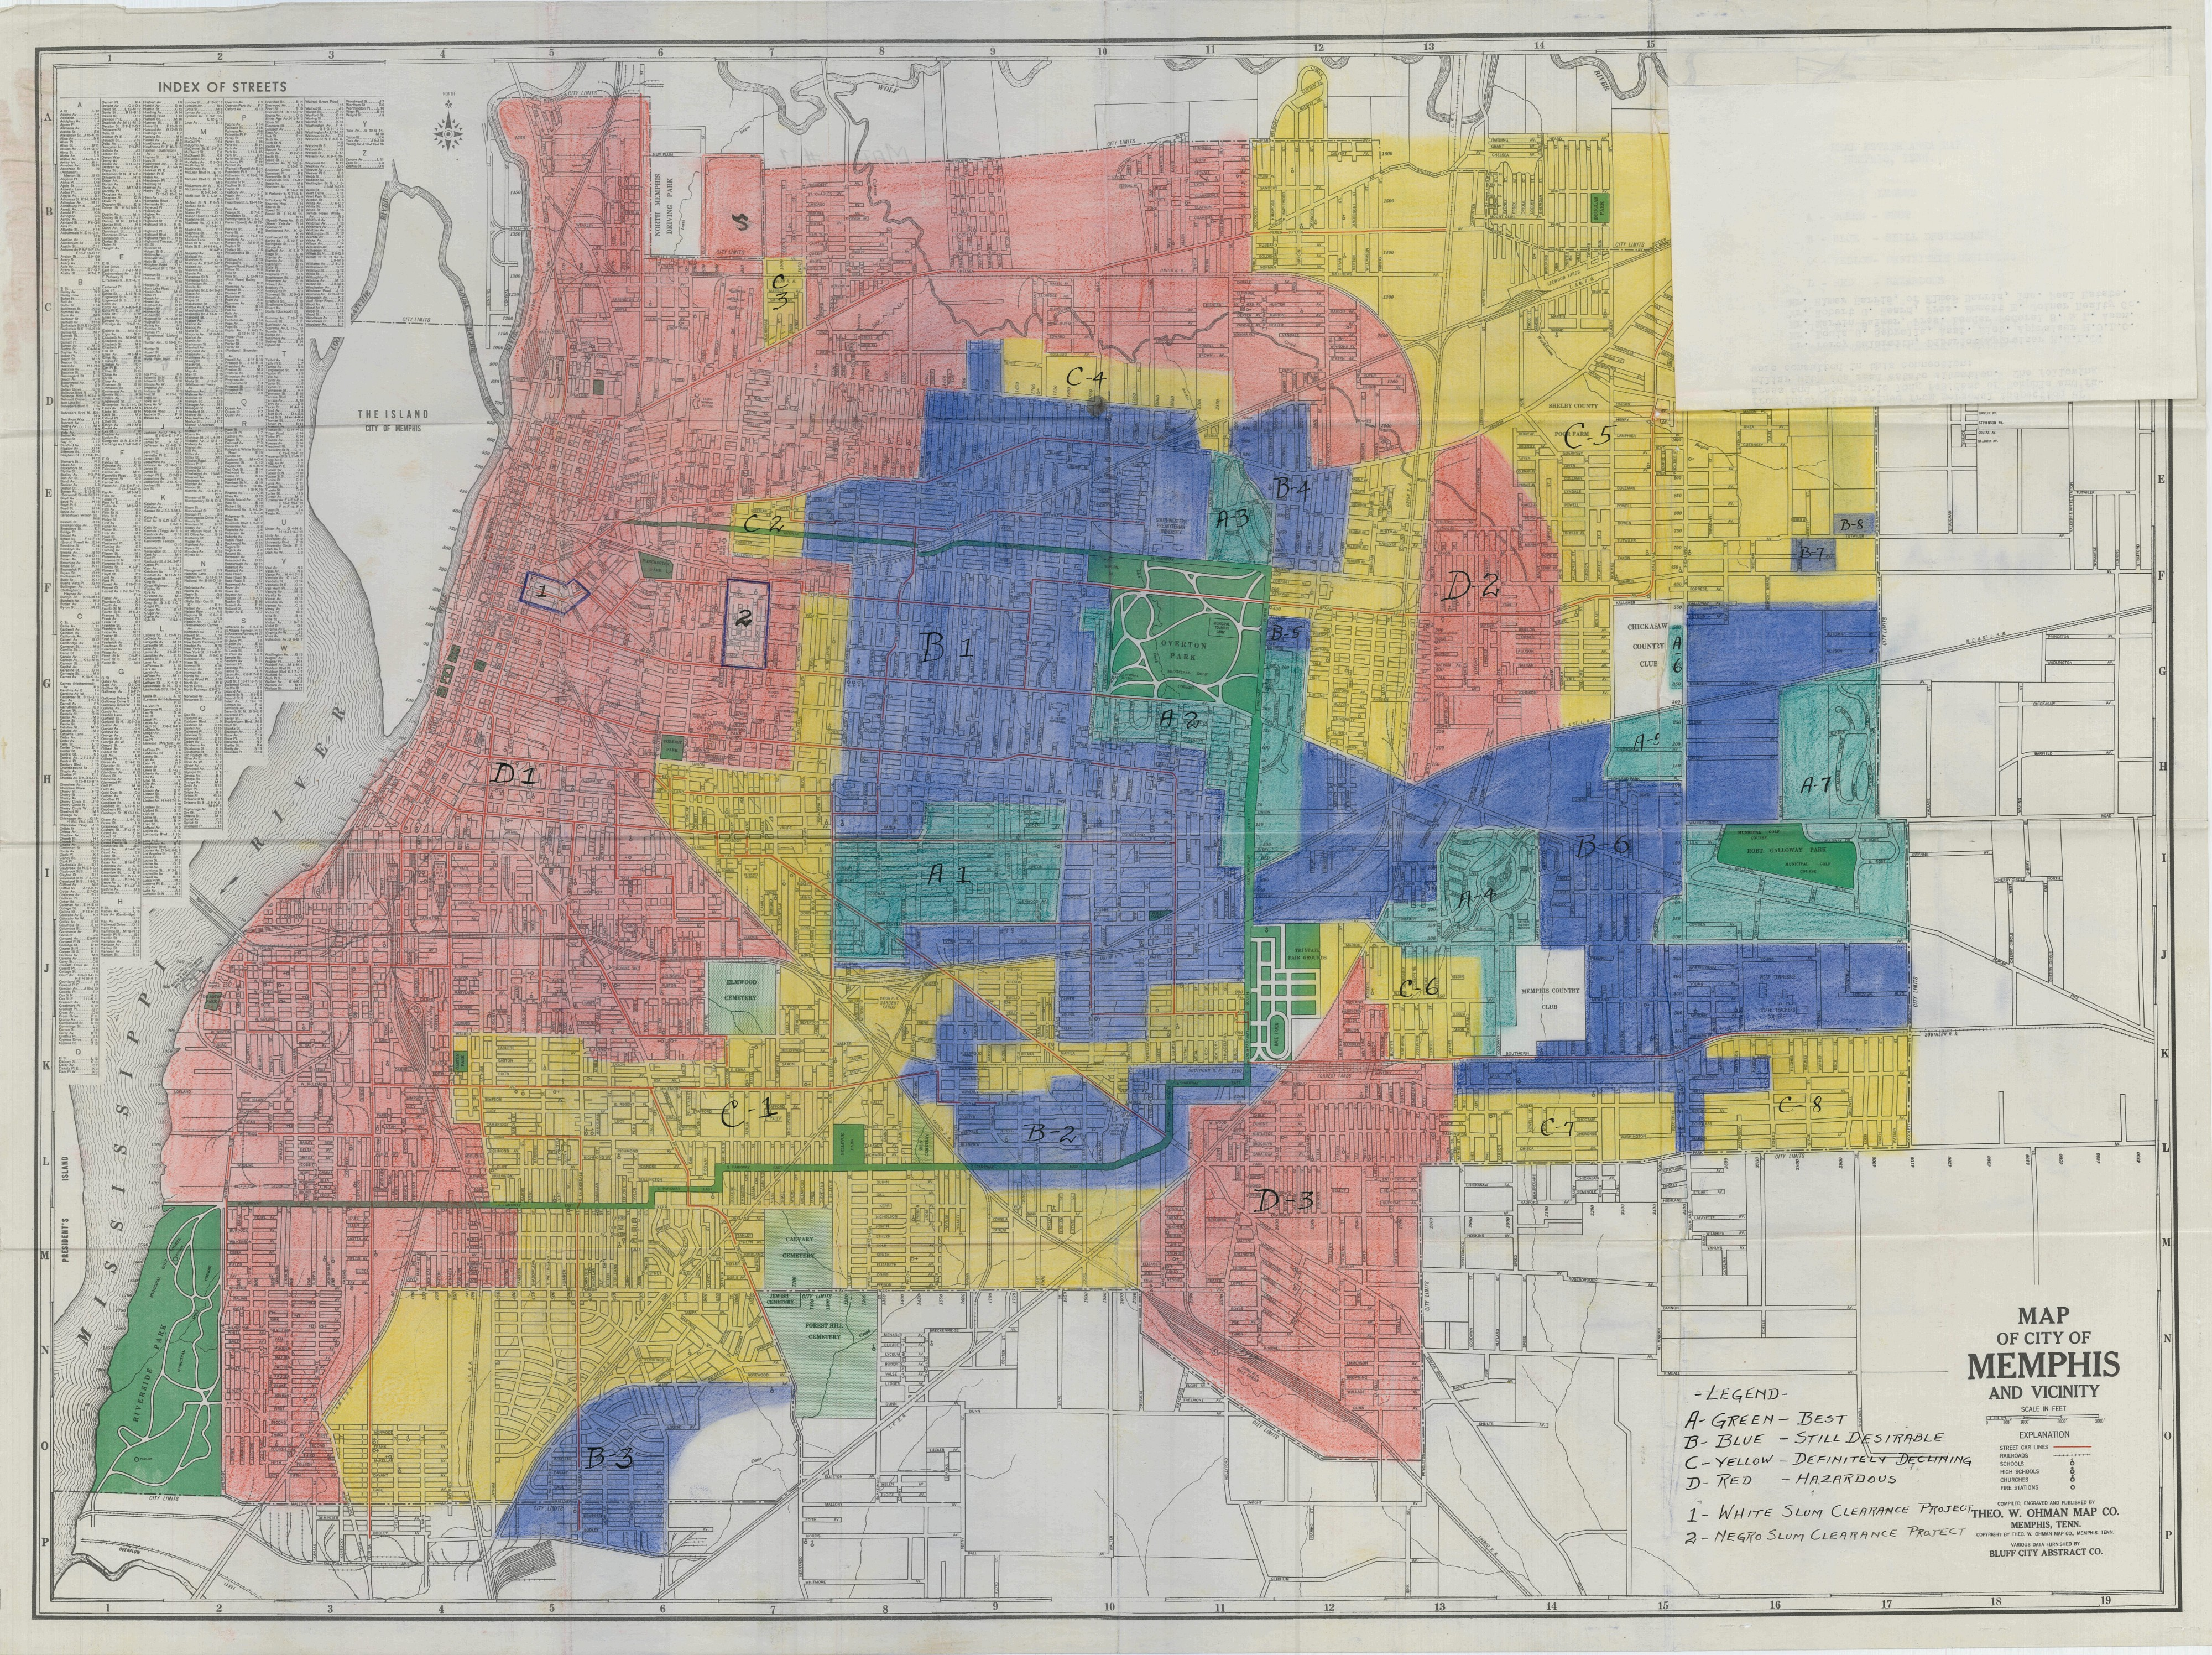
\includegraphics{_img/memphis_redliningmap.jpg}
\caption[A color-coded map of Memphis created in the 1930s used by the federal government to rate mortgage risk. Original source: National Archives and Records Administration, accessed via.]{A color-coded map of Memphis created in the 1930s used by the federal government to rate mortgage risk. Original source: National Archives and Records Administration, accessed via.\footnotemark{}}
\end{figure}
\footnotetext{\protect\hyperlink{ref-bradley2019}{Cole Bradley, {``Seeing Red I: Mapping 90 Years of Redlining in Memphis,''} March 31, 2019, \url{https://www.highgroundnews.com/features/SeeingRedlining.aspx}}.}

A digitized version of the above map is available below.\footnote{I originally made this map using \href{https://geojson.io/}{geojson.io} for a class in spring 2021. I have since discovered the University of Richmond's \href{https://dsl.richmond.edu/panorama/redlining/\#loc=5/39.1/-94.58}{Mapping Inequality} website, which offers original scans and digitized versions (geoJSON or shapefiles) of redlining maps available for download for over 100 U.S. cities.}

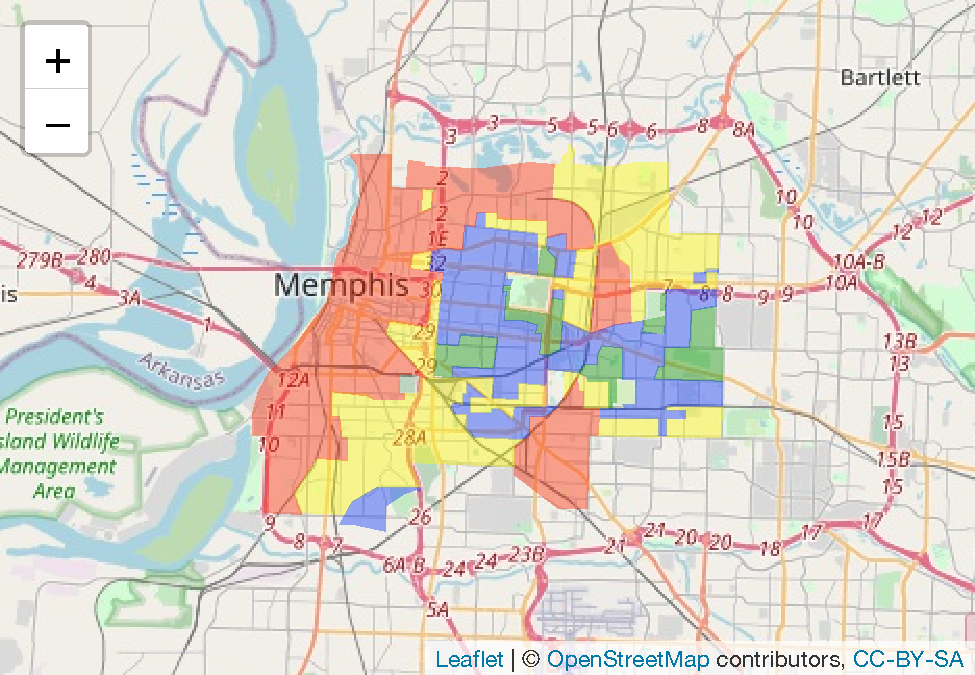
\includegraphics{MA-capstone_files/figure-latex/redlineLeaflet-1.pdf}

Overall, 69\%\footnote{Percentages sourced from (\protect\hyperlink{ref-nelson}{Robert K. Nelson et al., {``Mapping Inequality,''} n.d., \url{https://dsl.richmond.edu/panorama/redlining/}}).} of the city was deemed ``hazardous'' (red) or ``definitely declining'' (yellow), notably including all of Downtown and the majority of North and South Memphis. The federal government deemed these mortgages risky, and either denied the loan or charging higher rates to account for the ``risk.''

Only 7\% of the city received an A rating (``best,'' green), including the Central Gardens neighborhood, areas adjacent to Overton Park, Chickasaw Gardens, and East Memphis neighborhoods adjacent to golf courses. These neighborhoods have notably remained occupied and maintained over the decades.

The remaining 24\% of the city (``still desirable,'' blue) contains other Midtown neighborhoods and follows the Poplar Avenue corridor to the east, drawing residents toward the suburbs.

\hypertarget{modern-discrimination}{%
\subsection{Modern Discrimination}\label{modern-discrimination}}

In recent years, at least three major lawsuits have been settled concerning discriminatory lending in Memphis.\footnote{\protect\hyperlink{ref-bradley2019}{Bradley, {``Seeing Red I''}}; \protect\hyperlink{ref-uhlmann2020}{Alexander Uhlmann, {``The State of Evictions in Memphis, Tennessee''} (University of Texas, Austin, December 2020)}.} Excessive foreclosures following the 2008 subprime mortgage crisis led Memphis and Shelby County to file suit against Wells Fargo for targeting Black neighborhoods for predatory lending practices, which the bank settled for \$425 million in 2012.\footnote{\protect\hyperlink{ref-rothacker2012}{Rick Rothacker, {``Wells Fargo Spending {\$}432 Million to End Lending Suit,''} \emph{Reuters}, May 30, 2012, \url{https://www.reuters.com/article/us-wellsfargo-settlement-idUSBRE84S1H620120530}}.}

Following the Great Recession, banks became selective of whom they targeted and approved for mortgages, often at the expensive of non-white residents. In 2016, BancorpSouth and First Tennessee Bank settled separate suits for \$10.6 million and \$1.9 million, respectively, against accusations of disproportionately denying loan applications to non-white borrowers and failing to build branches in non-white neighborhoods.\footnote{\protect\hyperlink{ref-lane2016a}{Ben Lane, {``BancorpSouth Fined {\$}10.6 Million for Discriminatory Lending, Redlining,''} June 29, 2016, \url{https://www.housingwire.com/articles/37405-bancorpsouth-fined-106-million-for-discriminatory-lending-redlining/}}; \protect\hyperlink{ref-lane2016}{Ben Lane, {``First Tennessee Bank Reaches {\$}1.9 Million Settlement over Discriminatory Lending,''} February 1, 2016, \url{https://www.housingwire.com/articles/36175-first-tennessee-bank-reaches-19-million-settlement-over-discriminatory-lending/}}.}

\hypertarget{health-healthy-homes}{%
\section{Health \& Healthy Homes}\label{health-healthy-homes}}

In 2015, Memphis was named the asthma capital of America by the Asthma and Allergy Foundation of America,\footnote{\protect\hyperlink{ref-aafa2015}{AAFA, {``Asthma Capitals 2015,''} 2015, \url{https://www.aafa.org/media/1607/asthma-capitals-report-2015-rankings.pdf}}.} based on prevalence, risk factors, and medical factors. Recent efforts to reduce the prevalence and risk of asthma have been successful---Memphis's rank has since decreased to 41st in 2021.\footnote{\protect\hyperlink{ref-aafa2021}{AAFA, {``Asthma Capitals 2021: The Most Challenging Places to Live in with Asthma,''} 2021, \url{https://www.aafa.org/media/3040/aafa-2021-asthma-capitals-report.pdf}}.}\footnote{The ranking method changed between 2015 and 2021, with fewer factors involved in a city's overall ranking in 2021.} However, Memphis still ranks high in asthma-related mortality, placing 7th of 100 cities. A recent study comparing pediatric asthma data with property quality information found that asthma prevalence is disproportionately distributed throughout Memphis.\footnote{\protect\hyperlink{ref-shin2018}{Eun Kyong Shin and Arash Shaban-Nejad, {``Urban Decay and Pediatric Asthma Prevalence in Memphis, Tennessee: Urban Data Integration for Efficient Population Health Surveillance,''} \emph{IEEE Access} 6 (2018): 46281--89, doi:\href{https://doi.org/10.1109/ACCESS.2018.2866069}{10.1109/ACCESS.2018.2866069}}.} Neighborhood blight and inequality were closely associated with childhood asthma and other health problems.

In the Memphis area, the Healthy Homes Rating System has been used by inspectors with the Shelby County Department of Housing. The agency's Lead Hazard Reduction Program remediates homes with elevated lead levels. Funding is provided by HUD, and prior to beginning repairs, HUD requires the home be inspected for health hazards. Any funds leftover from lead remediation can be used towards improving Healthy Home violations.

\hypertarget{code-enforcement}{%
\section{Code Enforcement}\label{code-enforcement}}

Over the past twenty years, there have been at least two expansive reports offering critiques and criticisms of Memphis code enforcement.

The first report, released in April 2001, was distributed by the Memphis Shelby Crime Commission and written by Phyllis Betts, then a professor of sociology at University of Memphis.\footnote{\protect\hyperlink{ref-betts2001}{Phyllis Betts, {``Best Practice Number Ten: Fixing Broken Windows {{}} Strategies to Strengthen Housing Code Enforcement and Related Approaches to Community-Based Crime Prevention in Memphis,''} April 2001, \url{https://www.pdffiller.com/20879259-BestPracticeNumber10Fixing_Broken_Windowspdf-Best-Practice-Number-Ten-Center-For-Community-Building-and-cbana-memphis-}}.} Input was provided by two other University of Memphis faculty: Betts's husband, the late Richard Janikowski, former chair of the Department of Criminology and Criminal Justice and `father' of Memphis's Blue CRUSH policing;\footnote{\protect\hyperlink{ref-poe2021}{Ryan Poe, {``Richard Janikowski, 'Father' of Memphis' Blue CRUSH Model of Policing, Dies at 69,''} \emph{The Commercial Appeal}, March 24, 2021, \url{https://www.commercialappeal.com/story/news/local/2021/03/24/richard-janikowski-father-memphis-blue-crush-model-policing-dies-age-69/6966107002/}}.} and Susan Roakes, former professor of City and Regional Planning.

The report was built on the ``broken windows'' criminology theory: in deteriorated or declining neighborhoods, physical neglect of ``problem properties'' attracts and aggravates criminal activity.\footnote{\protect\hyperlink{ref-betts2001}{Betts, {``Best Practice Number Ten''}}.} Researchers interviewed inspectors and individuals involved with environmental court, used code enforcement data from 1992-1999, accessed the Shelby County Tax Assessor's database, and conducted visual surveys for selected properties as part of a case study of the Binghamton neighborhood.

The second report, published in 2018, was produced by The Urban Institute.\footnote{\protect\hyperlink{ref-stacy2018}{Christina Plerhoples Stacy, Joseph Schilling, and Steve Barlow, {``Strategic Housing Code Enforcement and Public Health,''} October 17, 2018, \url{https://www.urban.org/research/publication/strategic-housing-code-enforcement-and-public-health}}.} While the 2001 report focused on property neglect and \emph{safety}, this report centered on the link between the physical condition of homes and neighborhoods and \emph{public health}. Planning for the report began shortly after the election of Mayor Jim Strickland in 2016, whose campaign had emphasized blight control.\footnote{\protect\hyperlink{ref-baker2018}{Jackson Baker, {``The First 1000 Days of Jim Strickland,''} \emph{Memphis Magazine}, September 3, 2018, \url{https://memphismagazine.com/api/content/65e8dd62-aae1-11e8-9153-120e7ad5cf50/}}.} Researchers collaborated with and interviewed members of the newly formed \href{http://memphisfightsblight.com/blight-elimination-steering-team/}{Blight Elimination Steering Team}, a coordinated effort between public, private, and nonprofit agencies to address blight, and the \href{https://www.greenandhealthyhomes.org/location/memphis-tn/}{Green and Healthy Homes Initiative}, a partnership formed between local health care providers and housing and community development organizations to address public health issues related to housing quality.

The Urban report accessed and analyzed data through the \href{http://memphisfightsblight.com/programs/mph/}{Memphis Property Hub}, which offers parcel-level property information, particularly related to blighted, vacant, and foreclosed homes. Code enforcement data from 1999-2017 was used, effectively picking up where the last report ended. Additional data related to public health, safety, and courts were provided by the Shelby County Healthy Department, the Center for Applied Earth Science and Engineering Research department at the University of Memphis, and the Shelby County Environmental Court, respectively.

\hypertarget{findings-and-recommendations}{%
\subsection{Findings and Recommendations}\label{findings-and-recommendations}}

Despite nearly twenty years difference, the reports contain similar finding and recommendations. Notably, each report recommended fundamentally changing Memphis code enforcement from a reactive process (responding to citizen reports) to a proactive, strategic system. This was largely due to the large volume of cases processed related to vehicle violations or weeds, rather than more serious violations.

Both reports found the vast majority of code enforcement reports were related to nonstructural issues. \protect\hyperlink{ref-betts2001}{Betts}\footnote{\protect\hyperlink{ref-betts2001}{{``Best Practice Number Ten''}}.} reported three out of four properties were cited for non-structural problems such as weeds, junk, and inoperable or abandoned vehicles. It appears this percentage has actually increased overtime; \protect\hyperlink{ref-stacy2018}{Stacy, Schilling, and Barlow}\footnote{\protect\hyperlink{ref-stacy2018}{{``Strategic Housing Code Enforcement and Public Health''}}.} stated 81\% of all requests concerned the yard or property, rather than the house.

\protect\hyperlink{ref-stacy2018}{Stacy, Schilling, and Barlow}\footnote{\protect\hyperlink{ref-stacy2018}{ibid.}} found service requests were concentrated in areas with single-family homes, and though about half of all requests were for multifamily units, most of these (70 percent) were for duplexes rather than apartment complexes. \protect\hyperlink{ref-betts2001}{Betts}\footnote{\protect\hyperlink{ref-betts2001}{{``Best Practice Number Ten''}}.} also found that large multifamily units flew under the radar; at least half of multifamily properties in Binghamton had violations in multiple units, yet code enforcement recorded only eight violations out of 1200 apartment units.

When the report's findings differed, it was usually due to increased workload. The number of service requests has appeared to increase overtime. In 1998, code enforcement received about 10,000 complaints,\footnote{\protect\hyperlink{ref-betts2001}{Ibid., 93}.} while the Urban Institute reported 53,226 in 2016.\footnote{\protect\hyperlink{ref-stacy2018}{Stacy, Schilling, and Barlow, {``Strategic Housing Code Enforcement and Public Health,''} 51}.} However, this number does not match a dataset from the City of Memphis (discussed later in this paper) which reported 30,361 requests in 2016, not excluding duplicates. Nevertheless, it does appear that more requests are being made.

Newer cases also appear significantly more likely to be taken to court. In 1998, a mere 71 cases from code enforcement were heard by the environmental court.\footnote{\protect\hyperlink{ref-betts2001}{Betts, {``Best Practice Number Ten,''} 49}.} In November 2017 alone, 1,095 cases went to environmental court, though the Urban report does not specifically state if all cases were from code enforcement.\footnote{\protect\hyperlink{ref-stacy2018}{Stacy, Schilling, and Barlow, {``Strategic Housing Code Enforcement and Public Health,''} 51}.} The majority of new cases were for single-family homes (64\%), and most were vacant.

\protect\hyperlink{ref-stacy2018}{Stacy, Schilling, and Barlow}\footnote{\protect\hyperlink{ref-stacy2018}{{``Strategic Housing Code Enforcement and Public Health''}}.} suggests that code enforcement prioritize health-related violations and interior health and safety issues, cemented through the agency's policies and procedures manual. The authors recommend proactive inspections of problem multifamily properties and under-served neighborhoods, and identification of under-reported violations. Multiple technology improvements are recommended, including automatic prioritization of health-related violations and synchronizing of data systems with the Shelby County Department of Health and the environmental court, among others. Also acknowledged is the need to update current landlord/tenant laws to protect tenants from homelessness.

\hypertarget{census-data}{%
\chapter{Census Data}\label{census-data}}

Memphis is located on the bluffs of the Mississippi River in the southwest corner of Tennessee, adjacent to Mississippi and Arkansas. As such, the Memphis MSA includes counties in three states.

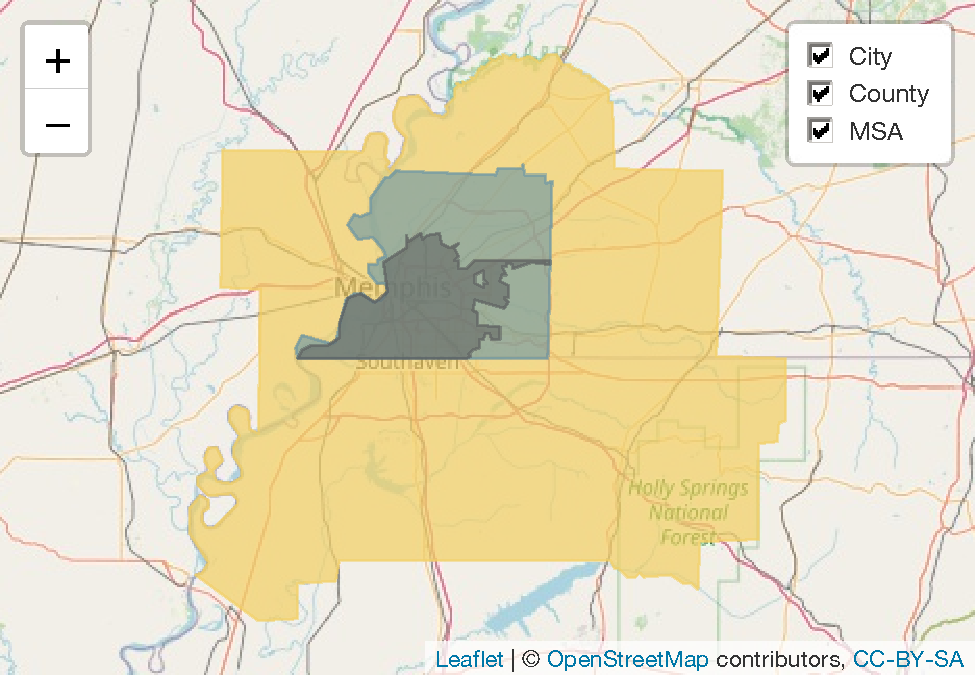
\includegraphics{MA-capstone_files/figure-latex/mapboundaries-1.pdf}

Boundaries for Memphis were downloaded from \href{https://data.memphistn.gov/dataset/Jurisdiction-Boundary-Memphis/b9uj-qyia}{Memphis Data Hub}, and for Shelby County and Memphis MSA from \href{https://geoportal.memphis.edu/}{CAESAR Geoportal}.

\hypertarget{summary-data}{%
\section{Summary Data}\label{summary-data}}

The American Community Survey (ACS) collects yearly data on population and housing in large metro areas. In 2019, the ACS reported there were 651,932 people living in the city of Memphis. Of this population, 15,843 were living in group quarters\footnote{The census divides group quarters into institutionalized facilities (nursing, adult correctional, and juvenile) and non-institutionalized facilities (university student housing and military quarters).}; the remaining 636,089 were occupying 251,732 housing units. The city also had 48,181 vacant units, for a total 299,913 housing units.

This information is shown in the following table, sorted by how these figures have changed since 2010.

\begin{table}

\caption{\label{tab:pophsgdifference}Population and housing data, Memphis}
\centering
\begin{tabular}[t]{l|r|r}
\hline
Variable & 2019 Estimate & Change from 2010-2019\\
\hline
Occupied Housing Units & 251,732 & 5,237\\
\hline
Total Housing Units & 299,913 & 3,895\\
\hline
Population Living in Occupied Housing Units & 636,089 & -355\\
\hline
Vacant Housing Units & 48,181 & -1,342\\
\hline
Population Living in Group Quarters & 15,843 & -2,589\\
\hline
Total Population & 651,932 & -2,944\\
\hline
\end{tabular}
\end{table}

From 2010 to 2019, Memphis's population decreased by about 2,944 people. Most of this was a decrease in the number of people living in group quarters (2,589); the population living in occupied units only decreased by 355 individuals over this period. Overall, the population is stagnant.

During this time, the total number of housing units increased by 3,895. Considering the population changes, we might expect this to be accompanied with an increase in vacancies and decrease in the number of occupied units, yet neither happened. The number of vacant units decreased by 1,342 and the number of occupied units increased by 5,237.

This is an interesting phenomenon: an increase of 5,237 units that are occupied, and a decrease of 355 people living in occupied units. One possible explanation is a change in how many people live together, such as two people living together in 2010 who lived apart in 2019. Considering the trend at a city-wide level, this could be explained by a decrease in the number of families and an increase in the number of people living alone. We can confirm/disprove this using ACS data on household size.

\begin{table}

\caption{\label{tab:tenhhsizetbl}Change in household size by tenure, 2010-2019, Memphis}
\centering
\begin{tabular}[t]{l|r|r|r}
\hline
Household Size & Owner & Renter & Total Change\\
\hline
1-person household & -1,347 & 11,766 & 10,419\\
\hline
2-person household & -3,481 & 7,628 & 4,147\\
\hline
3-person household & -3,463 & 367 & -3,096\\
\hline
4-person household & -3,080 & 1,540 & -1,540\\
\hline
5-person household & -2,737 & -585 & -3,322\\
\hline
6-person household & -245 & 36 & -209\\
\hline
7-or-more person household & -724 & -438 & -1,162\\
\hline
\end{tabular}
\end{table}

The data appears to confirm this hypothesis. From 2010 to 2019, the number of 2+ person households dropped by 5,182, and the number of 1-person households increased by 10,419. These are significant changes for a stagnant population.

The above table also shows that Memphis's change in household size has been significantly linked to tenure. During the 2010s, the city lost owner-occupied households at every household size, for a combined loss of 15,077 households. Over the same period, Memphis gained 20,314 renting households, who were mostly 1 or 2 people living together. The change in renters and owners totals an overall gain of 5,237 households.

When did this change happen? Are the renters former owners? From out of state? Kids moving out of their parents home? Let's delve deeper into changes in tenure over the past year.

\hypertarget{changes-in-tenure}{%
\section{Changes in Tenure}\label{changes-in-tenure}}

\hypertarget{housing-characteristics}{%
\section{Housing Characteristics}\label{housing-characteristics}}

Of occupied homes in 2019, 117,361 (47\%) were owner-occupied; 134,371 (53\%) were renter-occupied.

\hypertarget{median-year-built}{%
\subsection{Median Year Built}\label{median-year-built}}

The age of a housing unit can be an indicator that repairs are needed. The below table shows the median age of occupied housing units in the city of Memphis, separated by tenure.

\begin{table}

\caption{\label{tab:tblmedyrbltmem}Median year built of occupied housing units in City of Memphis}
\centering
\begin{tabular}[t]{l|c|c}
\hline
Census Year & Owner-Occupied & Renter-Occupied\\
\hline
2010 & 1966 & 1973\\
\hline
2011 & 1966 & 1973\\
\hline
2012 & 1966 & 1973\\
\hline
2013 & 1966 & 1973\\
\hline
2014 & 1966 & 1973\\
\hline
2015 & 1966 & 1973\\
\hline
2016 & 1966 & 1973\\
\hline
2017 & 1966 & 1973\\
\hline
2018 & 1966 & 1973\\
\hline
2019 & 1966 & 1974\\
\hline
\end{tabular}
\end{table}

The Memphis housing stock is aging. The median year built has not (or barely) budged over the past ten years for all occupied homes. The median age of owner-occupied homes is 55 years; for renter-occupied homes, 47 years. The median year built for both owner and renter occupied units is before the ban of lead-based paint in 1978, indicating many homes are at risk for lead poisoning if they have not been remediated.

When we expand our scope from the city limits to the Memphis MSA, there is a noticeable shift in the data, as seen in the table below.

\begin{table}

\caption{\label{tab:tblmedyrbltmsa}Median year built of occupied housing units in Memphis MSA}
\centering
\begin{tabular}[t]{l|c|c}
\hline
Census Year & Owner-Occupied & Renter-Occupied\\
\hline
2010 & 1982 & 1977\\
\hline
2011 & 1982 & 1977\\
\hline
2012 & 1983 & 1978\\
\hline
2013 & 1983 & 1978\\
\hline
2014 & 1983 & 1978\\
\hline
2015 & 1983 & 1978\\
\hline
2016 & 1984 & 1978\\
\hline
2017 & 1984 & 1978\\
\hline
2018 & 1984 & 1978\\
\hline
2019 & 1985 & 1978\\
\hline
\end{tabular}
\end{table}

In the MSA, the median age of renter-occupied homes is 43; for owner-occupied units, 36. This signifies that most new development in the MSA has been for owner-occupied homes outside city limits. We can confirm this by looking at more detailed data available from the Census.

\hypertarget{year-structure-built}{%
\subsection{Year Structure Built}\label{year-structure-built}}

The following graph shows the number of homes built each year in Memphis, separated by tenure.

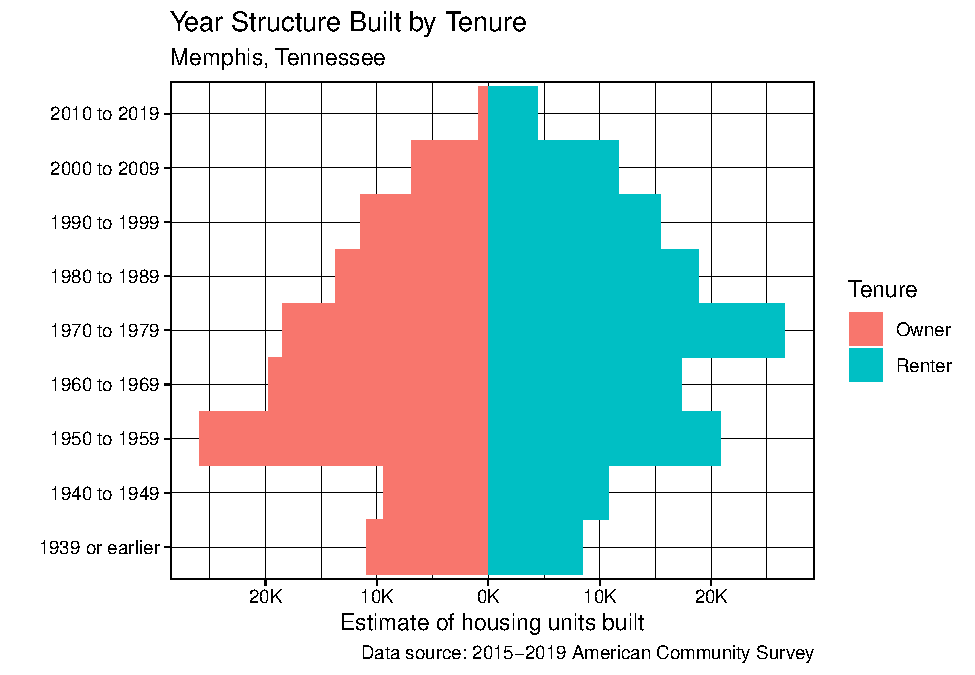
\includegraphics{MA-capstone_files/figure-latex/ggplotysb-1.pdf}

More owner-occupied homes were built between 1950 to 1959 than any other period, with the stock gradually decreasing every decade since, plummeting after 2010. According to the data, there are \textbf{only 872 owner-occupied homes constructed since 2010}. It is now clear why the median year built for these homes has not budged in the past decade.

The year renter-occupied homes were built peaked in the 1970s, eclipsing owner-occupied homes and outpacing it ever since (though still declining). Rental homes also sharply decrease after 2010, but not as severe. Of occupied rental homes, \textbf{4,404 were constructed since 2010}.

Note that this dataset shows the year homes were built based on \textbf{current} tenure. It is possible for a home to originally have been owner-occupied and converted to a rental. We can investigate this by comparing 2015-2019 ACS data with 2005-2009 data and measuring the difference.

\begin{table}

\caption{\label{tab:tbl-yrblt-diff}Change in Occupied Units by Year Structure Built from 2009 to 2019 ACS}
\centering
\begin{tabular}[t]{l|c|c|c}
\hline
Year Structure Built & Owner & Renter & All Occupied Units\\
\hline
Built 1939 or earlier & -2796 & -848 & -3644\\
\hline
Built 1940 to 1949 & -2479 & 2111 & -368\\
\hline
Built 1950 to 1959 & -5452 & 4241 & -1211\\
\hline
Built 1960 to 1969 & -4411 & -179 & -4590\\
\hline
Built 1970 to 1979 & -4882 & 1654 & -3228\\
\hline
Built 1980 to 1989 & -3290 & 110 & -3180\\
\hline
Built 1990 to 1999 & -1876 & 2624 & 748\\
\hline
Built 2000 to 2009 & -281 & 2113 & 1832\\
\hline
\end{tabular}
\end{table}

There was an overall loss of 13,641 occupied housing units between 2009-2019 in the city of Memphis. Broken down by tenure, there was a loss of 25,467 owner-occupied units, and a gain of 11,826 renter occupied units. If we limit our scope to \textbf{``older'' units (built before 1990)}, there was a \textbf{loss of 23,310 owner-occupied units}, and a \textbf{gain of 7,089 renter-occupied units}.

We would expect a loss in older housing units over time, as we cannot travel back in time and create more units.\footnote{The gain of units from 1990 to 1999 is likely due to data error. Another explanation is that previously vacant units built during this time are now occupied. But this is unlikely given the loss in occupied units and an increase in vacant units from 2009-2019.} This is true overall, but we can see that large losses in owner-occupied units are partially offset by gains in renter-occupied units. This tells us formerly owner-occupied homes have converted into rentals.

Considering the Great Recession, this implies former homeowners are now renting. Households that formerly benefited from policies and programs geared toward homeowners now navigate a housing system that is decidedly anti-renter. They lost their opportunity to build generational wealth, and now their wealth is being extracted through rents. Additionally, homes being converted into rentals limits the availability of homes for purchase, and denies young people the opportunity to plant roots in the community.

Below is a graph visualizing the above table.

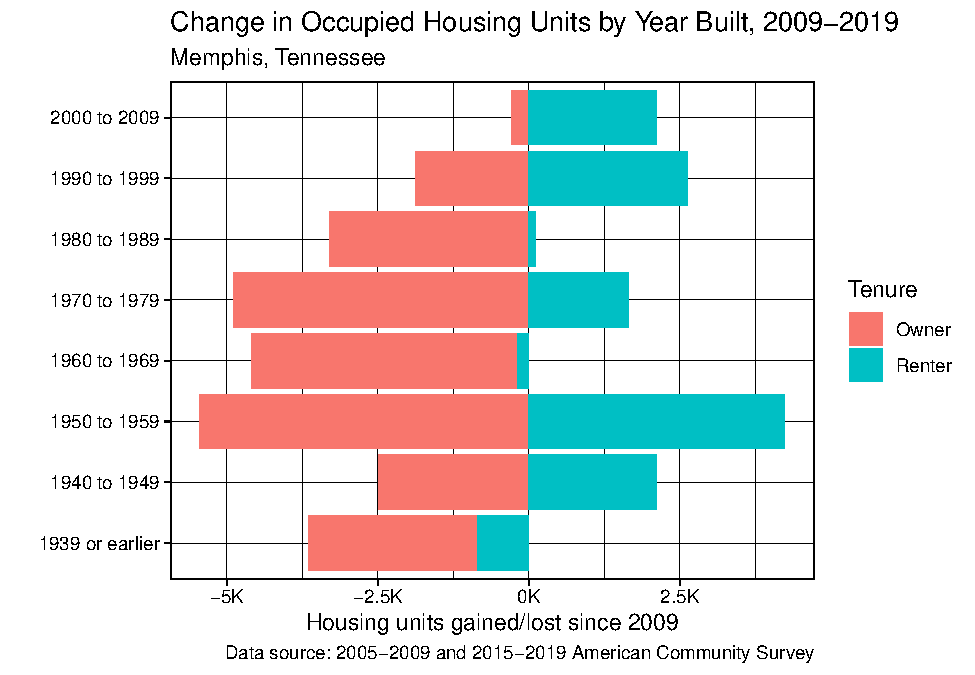
\includegraphics{MA-capstone_files/figure-latex/ggplotdec-1.pdf}

Between the 2009 and 2019 ACS, there was a definite loss in occupied housing units built before 1939 and between 1960-1969. In every other decade, there was a loss of owner-occupied units and a gain in renter-occupied units. As we cannot travel back in time and build more rental units, we can assume that these were formerly owner-occupied units that have been converted to rental units.

\hypertarget{housing-quality}{%
\section{Housing Quality}\label{housing-quality}}

Data on housing quality in the Memphis MSA is available through the 2019 \href{https://www.census.gov/programs-surveys/ahs.html}{American Housing Survey}. As the median age for rental homes is seven years older than for owner-occupied homes in the MSA, we can expect renter-occupied homes to have more deficiencies and problems than owner-occupied homes.

When surveyed on the adequacy of their housing, 14.5\% of renter-occupied units were thought of as inadequate, compared to 10\% of owner-occupied units. This disparity in quality between renter- and owner-occupied households is significant when we compare specific housing problems, as shown in the tables below.\footnote{In the discussions below, ``renters'' refers to renter-occupied units, ``owners'' refers to owner-occupied units, and ``Memphis'' refers to the Memphis MSA.}

\hypertarget{selected-housing-deficiencies}{%
\subsection{Selected Housing Deficiencies}\label{selected-housing-deficiencies}}

\begin{table}

\caption{\label{tab:tbl-AHSselfdef}Selected Housing Deficiencies, Memphis MSA}
\centering
\begin{tabular}[t]{l|c|c|c|c|c|c}
\hline
\multicolumn{1}{c|}{ } & \multicolumn{2}{c|}{Rent} & \multicolumn{2}{c|}{Own} & \multicolumn{2}{c}{All} \\
\cline{2-3} \cline{4-5} \cline{6-7}
Deficiency & est. & \% & est. & \% & est. & \%\\
\hline
Signs of mice or rats inside home in last 12 months & 24.4 & 10.89\% & 32.6 & 11.25\% & 56.9 & 11.08\%\\
\hline
Signs of cockroaches in last 12 months & 50.9 & 22.72\% & 44.4 & 15.33\% & 95.3 & 18.55\%\\
\hline
Holes in floors & NA & NA & NA & NA & 4.2 & 0.82\%\\
\hline
Open cracks or holes (interior) & 14.4 & 6.43\% & 12.1 & 4.18\% & 26.6 & 5.18\%\\
\hline
Broken plaster or peeling paint (interior) & 5.3 & 2.37\% & 5.8 & 2\% & 11.1 & 2.16\%\\
\hline
Exposed wiring & 3.9 & 1.74\% & 4.5 & 1.55\% & 8.4 & 1.64\%\\
\hline
Rooms without electric outlets & 6.6 & 2.95\% & 5.0 & 1.73\% & 11.6 & 2.26\%\\
\hline
\end{tabular}
\end{table}

\emph{Source: \href{https://www.census.gov/newsroom/press-releases/2020/2019-american-housing-survey.html}{American Housing Survey} (2019). Estimates in thousands of housing units.}

Renter-occupied units experienced more housing deficiencies than owner-occupied units for all but one of the selected problems.

Pests are prevalent in both owner and renter-occupied units. Renters saw more signs of cockroaches (by 7.4 percentage points), while owners were more likely to sight mice or rats (by 0.4 percentage points). These trends align with national data, where renters were 1.98 times more likely to see cockroaches and owners were 1.17 times more likely to report a rodent sighting.\footnote{\protect\hyperlink{ref-sellner2021}{Michael Sellner and Jordan Wicht, {``How Many American Homes Have Pests?''} April 21, 2021, \url{https://www.census.gov/library/stories/2021/04/how-many-american-homes-have-pests.html}}.} Compared to national averages, housing units in the Memphis MSA saw slightly fewer rodents (11.1\% vs 11.9\%) and significantly more cockroaches (18.6\% vs.~11.3\%).

Renters were moderately more likely to have open cracks or holes in the interior of their home and to have rooms without electrical outlets. They were also slightly more likely to have decaying interior walls and exposed wiring.

\hypertarget{housing-problems}{%
\subsection{Housing Problems}\label{housing-problems}}

The following table shows the number of units who experience selected housing problems. An estimate of ``S'' denotes a sample too small to meet publication standards or avoid disclosure of identifying information. The total column (``Tot'') is the number of housing units \emph{capable} of experiencing each problem (rather than all housing units). For instance, the total number of units with heating problems only includes units with heating equipment who occupied their unit last winter (excluding units without heating equipment or those who did not occupy their unit last winter).

\begin{longtable}[]{@{}lccccc@{}}
\caption{Selected Housing Problems}\tabularnewline
\toprule
& Rent & & & Own & \\
\midrule
\endfirsthead
\toprule
& Rent & & & Own & \\
\midrule
\endhead
\textbf{Problem} & \textbf{est.} & \textbf{\%} & & \textbf{est.} & \textbf{\%} \\
No flush toilet working some time in last 3 months & 7.0 & 3.1\% & & NA & NA \\
Uncomfortably cold for 24 hours or more & 12.3 & 6.6\% & & 10.8 & 3.9\% \\
Fuses or breakers blown in last 3 months & 14.1 & 6.3\% & & 19.3 & 6.7\% \\
Water stoppage in last 3 months & 6.4 & 2.9\% & & 3.2 & 1.1\% \\
Water leakage from inside structure & 19.5 & 8.7\% & & 20.7 & 7.1\% \\
Water leakage from outside structure & 18.9 & 8.4\% & & 25.5 & 8.8\% \\
Mold in last 12 months & 11.8 & 5.3\% & & 5.8 & 2.0\% \\
Public sewer breakdown in last 3 months & 5.1 & 2.3\% & & NA & NA \\
\bottomrule
\end{longtable}

\emph{Source: \href{https://www.census.gov/newsroom/press-releases/2020/2019-american-housing-survey.html}{American Housing Survey} (2019). Estimates in thousands of housing units.}

Renter-occupied units were overall more likely to experience housing problems and breakdowns than owner-occupied units.

The most common problem for renters and owners was water leakage during the past year. Owners were slightly more likely (by 0.4 percentage points) to experience leakage from outside the structure, such as from the roof, walls, closed windows, or doors. Renters were more likely (by 1.6 percentage points) to experience internal water leakage, such as from a leaky pipe, a broken water heater, or a backed up or overflown fixture. This is likely why renters were more likely to report mold growth within the past year (by 3.3 percentage points).

Heating problems causing households to be uncomfortably cold for at least a day were more common for renter-occupied units (by 2.7 percentage points). Renters were also more likely to experience sanitation problems barely reported by owners. This includes having a public sewer breakdown or having no working toilets at some point in the last three months.

Owners were slightly more likely to recently experience a blown fuse or breaker.

\hypertarget{external-building-conditions}{%
\subsection{External Building Conditions}\label{external-building-conditions}}

The following table shows the number of units experiencing external building problems. This table is limited to single-unit homes, \textbf{excluding multi-unit homes}. Homes with more than one unit are significantly more likely to be renter-occupied. As such, approximately 106,400 rental units were excluded from this table.

\begin{table}

\caption{\label{tab:unnamed-chunk-9}External Building Conditions, Memphis MSA}
\centering
\begin{tabular}[t]{l|c|c|c|c|c|c}
\hline
\multicolumn{1}{c|}{ } & \multicolumn{2}{c|}{Rent} & \multicolumn{2}{c|}{Own} & \multicolumn{2}{c}{All} \\
\cline{2-3} \cline{4-5} \cline{6-7}
Condition & est. & \% & est. & \% & est. & \%\\
\hline
Sagging roof & NA & NA & NA & NA & 7.4 & 1.83\%\\
\hline
Missing roofing material & 7.0 & 5.95\% & 15.5 & 5.4\% & 22.5 & 5.56\%\\
\hline
Hole in roof & 4.2 & 3.57\% & 6.2 & 2.16\% & 10.5 & 2.6\%\\
\hline
Missing bricks, siding, or other outside wall material & 3.9 & 3.32\% & 9.4 & 3.28\% & 13.3 & 3.29\%\\
\hline
Sloping outside walls & NA & NA & 4.5 & 1.57\% & 6.1 & 1.51\%\\
\hline
Broken windows & 7.6 & 6.46\% & 7.8 & 2.72\% & 15.4 & 3.81\%\\
\hline
Bars on windows & 16.1 & 13.69\% & 22.0 & 7.67\% & 38.1 & 9.42\%\\
\hline
Foundation crumbling or has open crack or hole & NA & NA & 14.5 & 5.05\% & 18.1 & 4.47\%\\
\hline
\end{tabular}
\end{table}

\emph{Source: \href{https://www.census.gov/newsroom/press-releases/2020/2019-american-housing-survey.html}{American Housing Survey} (2019). Estimates in thousands of housing units.}

Renters in single-unit homes were significantly more likely to experience external building problems than owner-occupied units, except for missing wall material, which afflicted 3.3\% of both renters and owners. Having bars on windows was especially more common in rental homes (by 9.0 percentage points), as well as having broken windows (by 3.8 percentage points). They were also slightly more likely to have roofing issues, such as missing roofing material or having a hole in the roof.

\hypertarget{data}{%
\chapter{311 Data}\label{data}}

Memphians are able to report problems to code enforcement by calling 311 or submitting a request through an app called \href{https://seeclickfix.com/}{SeeClickFix}, used in hundreds of towns across the nation.

Housing code enforcement data from 2016-present is available through \href{https://data.memphistn.gov/dataset/Service-Requests-since-2016/hmd4-ddta}{Memphis Data Hub}. This page uses a dataset downloaded July 19, 2021. At the time of download, there were 53 columns and 1,232,097 rows.

Considering the large number of rows and columns, this dataset might intimidate or dissuade individuals interested in the data who do not have the time to learn how to sort the data. Considering the extent of problems I had in parsing this data, I wanted to outline some basic advice and guidance for others interested in using this dataset.

R/RStudio was used to view and analyze the dataset, and all my code is available on the \href{https://github.com/sj-io/MA-capstone}{Github repository} for this paper. I set out with a goal to not manually edit the data (such as retyping individual cells) instead opting to use r packages like \href{https://dplyr.tidyverse.org/}{dplyr} to ``wrangle'' the data. This keeps the code reproducible, allowing anyone to download the newest 311 data and run it through the code to clean and organize it.

Each row of the 311 dataset contains all information for a single request, meaning there are not multiple rows for individual cases (except for duplicates).

Despite the large number of records, only a portion are relevant to this paper. This is because the dataset contains \textbf{all} requests to 311, not just those related to code enforcement. Additionally, many columns contain duplicate or unhelpful information. For instance, there are 23 columns related to location and under the column \texttt{LAST\_UPDATED\_BY}, every single entry is just the number ``460101.''

The dataset can be simplified by filtering for code enforcement data and narrowing the number of columns. The output is 14 columns and 154,844 rows, significantly easier to work with.

\begin{Shaded}
\begin{Highlighting}[]
\NormalTok{CE }\OtherTok{\textless{}{-}}\NormalTok{ Service\_Requests\_since\_2016 }\SpecialCharTok{\%\textgreater{}\%}
  \FunctionTok{filter}\NormalTok{(DEPARTMENT }\SpecialCharTok{==} \StringTok{"Code Enforcement"}\NormalTok{) }\SpecialCharTok{\%\textgreater{}\%}
  \FunctionTok{select}\NormalTok{(}
\NormalTok{    INCIDENT\_NUMBER, }\CommentTok{\#\textquotesingle{} service request (sr) number}
\NormalTok{    PARCEL\_ID, }\CommentTok{\#\textquotesingle{} parcel ID}
\NormalTok{    ADDRESS1, }\CommentTok{\#\textquotesingle{} the street name \& number}
\NormalTok{    REQUEST\_TYPE, }\CommentTok{\#\textquotesingle{} request category}
\NormalTok{    CE\_CATEGORY, }\CommentTok{\#\textquotesingle{} category for CE action}
\NormalTok{    RESOLUTION\_CODE}\SpecialCharTok{:}\NormalTok{RESOLUTION\_SUMMARY, }\CommentTok{\#\textquotesingle{} how the request resolved}
\NormalTok{    REQUEST\_STATUS, }\CommentTok{\#\textquotesingle{} open or closed?}
\NormalTok{    REPORTED\_DATE, }
\NormalTok{    LAST\_MODIFIED\_DATE, }
\NormalTok{    OWNER\_NAME, }\CommentTok{\#\textquotesingle{} assigned code inspector}
\NormalTok{    CREATED\_BY\_USER,}
\NormalTok{    location1 }\CommentTok{\#\textquotesingle{} geocoordinates}
\NormalTok{  ) }\SpecialCharTok{\%\textgreater{}\%} \FunctionTok{mutate}\NormalTok{(}\AttributeTok{RESOLUTION\_SUMMARY =} \FunctionTok{str\_to\_lower}\NormalTok{(RESOLUTION\_SUMMARY))}
\end{Highlighting}
\end{Shaded}

The above code chuck lists column names I kept which will be referenced below.

\hypertarget{problems-with-the-dataset}{%
\section{Problems with the dataset}\label{problems-with-the-dataset}}

Prior to analyzing this dataset, know that there are significant problems that need correcting, including inconsistent and vague data entry, hard-to-filter duplicates, an error causing the wrong address to appear, and more.

Throughout the dataset, there are \textbf{multiple values that mean the same thing}, like closed and resolved\footnote{Resolved has only been used 72 times, which begs the question of whether it needs to exist at all.}. The \texttt{RESOLUTION\_CODE} field in particular has a handful of codes used for an umbrella of meanings. For instance, 23\% of rows are resolved as ``NJ'' for Not Justified. This may mean an inspector has visited the property and did not see a problem, or there was a wrong address\footnote{INSUF (Insufficient information) is also used for wrong address cases.}, or there was a problem and it's been fixed, or there was a problem but it wasn't related to code enforcement; but in most cases there is no further explanation given. There are similar problems for codes tagged CVOM (COMP. V.O. - Miscellaneous, 9\% of all cases), CVOID (Closed Void, 4\% cases), CO (Closed Other, 3\%), and Other (1\%). Together, these codes make up \underline{40\%} of all code enforcement cases.

Another field with this problem is \texttt{REQUEST\_TYPE}. From 2016 to present, 29\% of all requests were simply listed as ``Code Miscellaneous.''

Some problems are caused by a \textbf{lack of updates} on behalf of inspectors. A file may never be closed in the system, even though the inspector is finished looking at the case. There are 779 active cases created in 2018 or earlier (at least 2.5 years old) and it is unclear if some are in a lengthy legal battle or were simply never updated.

There are many many \textbf{duplicated entries}. It's hard to determine exactly how many, because the duplicates will have unique values under \texttt{INCIDENT\_NUMBER} and slightly different date/times. For this reason it is hard to filter out without accidentally omitting multiple legitimate entries under the same property. Also, any entries that were created in error are kept in the system. This leads to inspectors frequently entering ``see sr\#xxxxxx'' in the \texttt{RESOLUTION\_SUMMARY}, referring to a different \texttt{INCIDENT\_NUMBER} that contains the correct file.\footnote{There are 6,391 instances of a \texttt{RESOLUTION\_SUMMARY} mentioning ``sr,'' and nearly all of these rows are likely to be duplicates.} There is also a code specifically for duplicate entries that already have an active file, JA (Justified, Active already file), which has been used 6,588 times, though other codes are known to be used for this same problem.

\textbf{Other problems are more major.} It appears that SeeClickFix (SCF), a program used to allow users to create requests, can cause the \textbf{wrong address} to be entered into the system. There is no warning given for this error. When I attempted to sort addresses with the most violations, the top address does not actually exist in the city of Memphis. The inspectors know this and they seem to be able to view the correct address in SCF, and sometimes (but not often) they will manually write this address in the \texttt{RESOLUTION\_SUMMARY}. It is unclear how many addresses have this problem, but it does affect multiple addresses. As a researcher, I feel nervous conducting research on data with such obvious errors.

Each row is meant to hold all information for a single case. There is also only one column for inspectors to manually enter notes: \texttt{RESOLUTION\_SUMMARY}. This column has become a \textbf{catch-all} for legitimate information, though it is also NA in 23\% of rows. In many other cases there is little elaboration, or the \texttt{RESOLUTION\_CODE\_MEANING} is simply repeated. Despite having eight different date columns, it is very common for dates to be entered here with the notes. Because this field is typed, typos are not-uncommon---tenant is spelled ``tennant'' 51 times, with many other variations such as ``tenenat,'' ``tenet,'' ``teneant'' and ``tenent.'' Other times a tenant is referred to as a ``resident.'' These variances make it difficult to find all instances of keywords.

Lastly, there are also obvious \textbf{privacy issues} included in the field, such as the full name and phone numbers of individuals.

\hypertarget{duplicates-errors}{%
\subsection{Duplicates \& Errors}\label{duplicates-errors}}

Searching for duplicates is made difficult by the large number of errors in the dataset. This is made clear when we begin searching for addresses with the most service requests.

\begin{verbatim}
## # A tibble: 6 x 2
##   ADDRESS1             n
##   <chr>            <int>
## 1 <NA>               547
## 2 746 CHAPEL ST      194
## 3 45 S IDLEWILD ST   117
## 4 1490 HUGENOT ST     88
## 5 3923 JACKSON AVE    76
## 6 102 PLAINVIEW ST    73
\end{verbatim}

There are 194 entries listed under the address 746 Chapel St, an address that does not seem to exist in Memphis (there is a Chapel \underline{Rd}, but no 746). Reviewing the \texttt{RESOLUTION\_SUMMARY} reveals the address to be a catch all of errors. Sometimes a different address or a business name is written in the \texttt{RESOLUTION\_SUMMARY}, indicating the results we are seeing is not the same as what was originally entered, yet code inspectors may be able to view the correct address. It is likely best to remove this address from any analysis involving location.

At 1490 Hugenot St, there are 117 requests, but this property appears to have the same problem as 746 Chapel. This is revealed by certain entries in the \texttt{RESOLUTION\_SUMMARY} including ``The correct address is xxx Summer Ave.'' and ``INSUFFICIENT INFORMATION WRONG ADDRESS SUBMITTED BY SEECLICKFIX'' (SeeClickFix, or SCF, is listed as the request creator for all but five entries at this address).

As for 45 S Idlewild, this is a valid location (an apartment complex) with 117 service requests. A closer look shows three people made 20 requests on February 1, 2019. Yet as discussed below, it is not clear if we should trust the information seen in \texttt{CREATED\_BY\_USER}.

When we look closer at \emph{who} is making complaints to code enforcement, it at first seems a few people are creating an astounding number of requests.\footnote{SCF stands for SeeClickFix, an app to create service requests.}

\begin{verbatim}
## # A tibble: 6 x 2
##   CREATED_BY_USER        n
##   <chr>              <int>
## 1 SCF                31585
## 2 HELEN.ANDERSON      6039
## 3 CAROLYN.FRANKLIN    5244
## 4 CHRISTINA.MCENTYRE  4708
## 5 ANGELA.HUMPHREY     4508
## 6 KRISTEN.PREWITT     3916
\end{verbatim}

However, filtering by HELEN.ANDERSON then ``tenant'' under \texttt{RESOLUTION\_SUMMARY} shows multiple instances where someone not named ``Helen Anderson'' is mentioned as the contact person across a wide variety of addresses. Further investigation found that some of the people listed as request creators are actually inspectors.

\hypertarget{basic-analysis}{%
\section{Basic Analysis}\label{basic-analysis}}

\hypertarget{number-of-requests}{%
\subsection{Number of Requests}\label{number-of-requests}}

Below is the number of requests for each year between 2016 and 2021, not excluding duplicates.

\begin{longtable}[]{@{}ll@{}}
\toprule
Reported Date & Number of Requests \\
\midrule
\endhead
2016 & 30,361 \\
2017 & 26,196 \\
2018 & 26,846 \\
2019 & 27,559 \\
2020 & 26,194 \\
2021 (as of 07/19/2021) & 17,688 \\
\bottomrule
\end{longtable}

The number of requests remained relatively constant over the years.

\hypertarget{active-cases}{%
\subsection{Active Cases}\label{active-cases}}

Below are cases that have not been marked ``Closed.''

\begin{longtable}[]{@{}ll@{}}
\toprule
Year & Active Cases \\
\midrule
\endhead
2016 & 136 \\
2017 & 111 \\
2018 & 532 \\
2019 & 956 \\
2020 & 1,098 \\
2021 & 5,630 \\
\textbf{All Years} & \textbf{8,463} \\
\bottomrule
\end{longtable}

According to the dataset, there are still 779 active cases from 2018 or earlier. However, many cases seem to have been simply abandoned.

\hypertarget{request-type}{%
\subsection{Request Type}\label{request-type}}

When a request is entered into 311, it must also be categorized. There are 14 categories for code enforcement data, including 3 categories related to COVID violations which were added in 2020. However, the vast majority of requests fell into one of five categories, listed below.

\begin{longtable}[]{@{}rllllllrl@{}}
\toprule
Request Type & 2016 & 2017 & 2018 & 2019 & 2020 & 2021 & All & Years \\
\midrule
\endhead
Code Miscellaneous & 28\% & 32\% & 32\% & 31\% & 25\% & 25\% & \textbf{45,028} & \textbf{29\%} \\
Vehicle Violation & 22\% & 26\% & 28\% & 26\% & 30\% & 35\% & \textbf{42,249} & \textbf{27\%} \\
Weeds Occupied & 20\% & 18\% & 17\% & 19\% & 14\% & 11\% & \textbf{26,161} & \textbf{17\%} \\
Junky Yard & 18\% & 13\% & 11\% & 12\% & 12\% & 15\% & \textbf{21,283} & \textbf{14\%} \\
Substandard, Derelict Structure & 9\% & 8\% & 10\% & 10\% & 7\% & 9\% & \textbf{13,778} & \textbf{9\%} \\
\textbf{Sum} & \textbf{97\%} & \textbf{97\%} & \textbf{98\%} & \textbf{98\%} & \textbf{88\%} & \textbf{95\%} & \textbf{148,499} & \textbf{96\%} \\
\bottomrule
\end{longtable}

From 2016 to 2019, more requests were sorted into ``Miscellaneous'' than any other category (surpassed by vehicle violations in 2020 and 2021). Considering that many cases related to housing are in this category, our job is made significantly harder. Rather that filtering and searching for a certain code, we are left to find these cases through a process of elimination.

\hypertarget{tidying-the-dataset}{%
\section{Tidying the Dataset}\label{tidying-the-dataset}}

After collecting basic information about the dataset, I began to sort the data into bins. I created bins for duplicates and errors, requests related to yards or cars, and other rows irrelevant to this research, like COVID mask violations.

Next I separated out rows where the \texttt{RESOLUTION\_SUMMARY} provided no new information (usually duplicating the \texttt{REQUEST\_CODE\_MEANING}.

I also separated rows related to the legal process into their own bin. As I separated out bins, I finally began to see rows related to housing. I created a ``building'' bin, and directed the code to include rows that mentioned words like ``roof,'' ``flooring,'' ``windows,'' or ``carpet,'' which can only refer to a structure.

I then began searching for rows related to ``tenant'' which also included ``moved'' or ``evict.'' Below is a table of such rows.

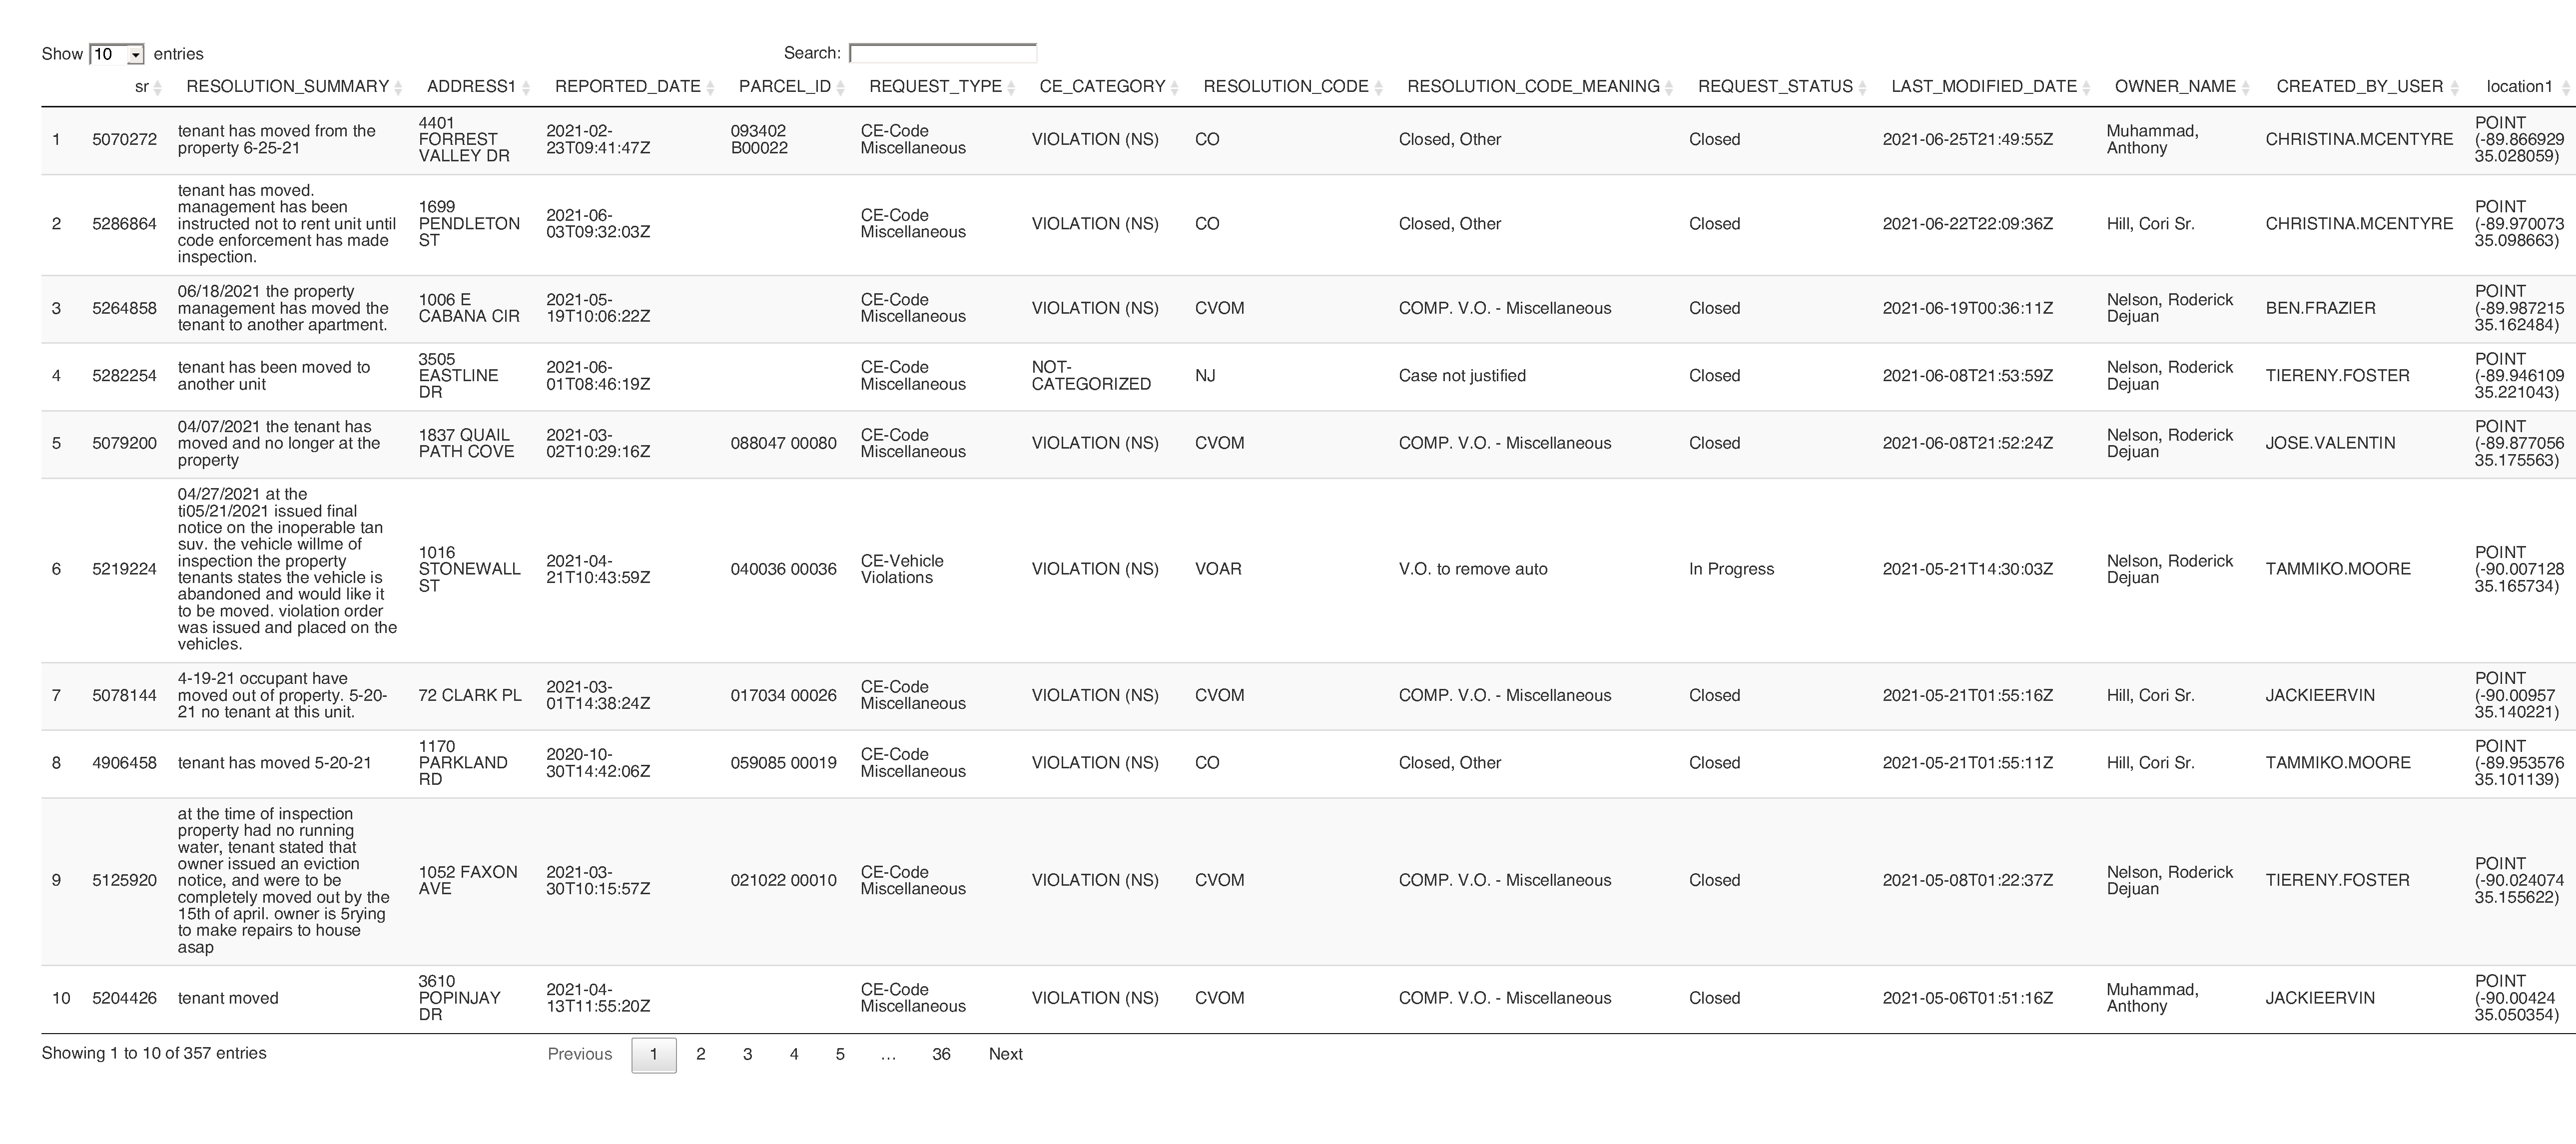
\includegraphics{MA-capstone_files/figure-latex/unnamed-chunk-15-1.pdf}

The vast majority of cases in the table are filed under ``Code Miscellaneous'' (305 of 357 rows). Clearly there is opportunity for a new \texttt{REQUEST\_TYPE} category to sort these rental-related cases.

In the above table, sr \#4569338 seems relevant to this paper

\begin{quote}
per: tenant jessica they moved due to respiratory problems from the mold/mildew like substance
\end{quote}

From here I created a separate table to search for rows related to ``mold.''

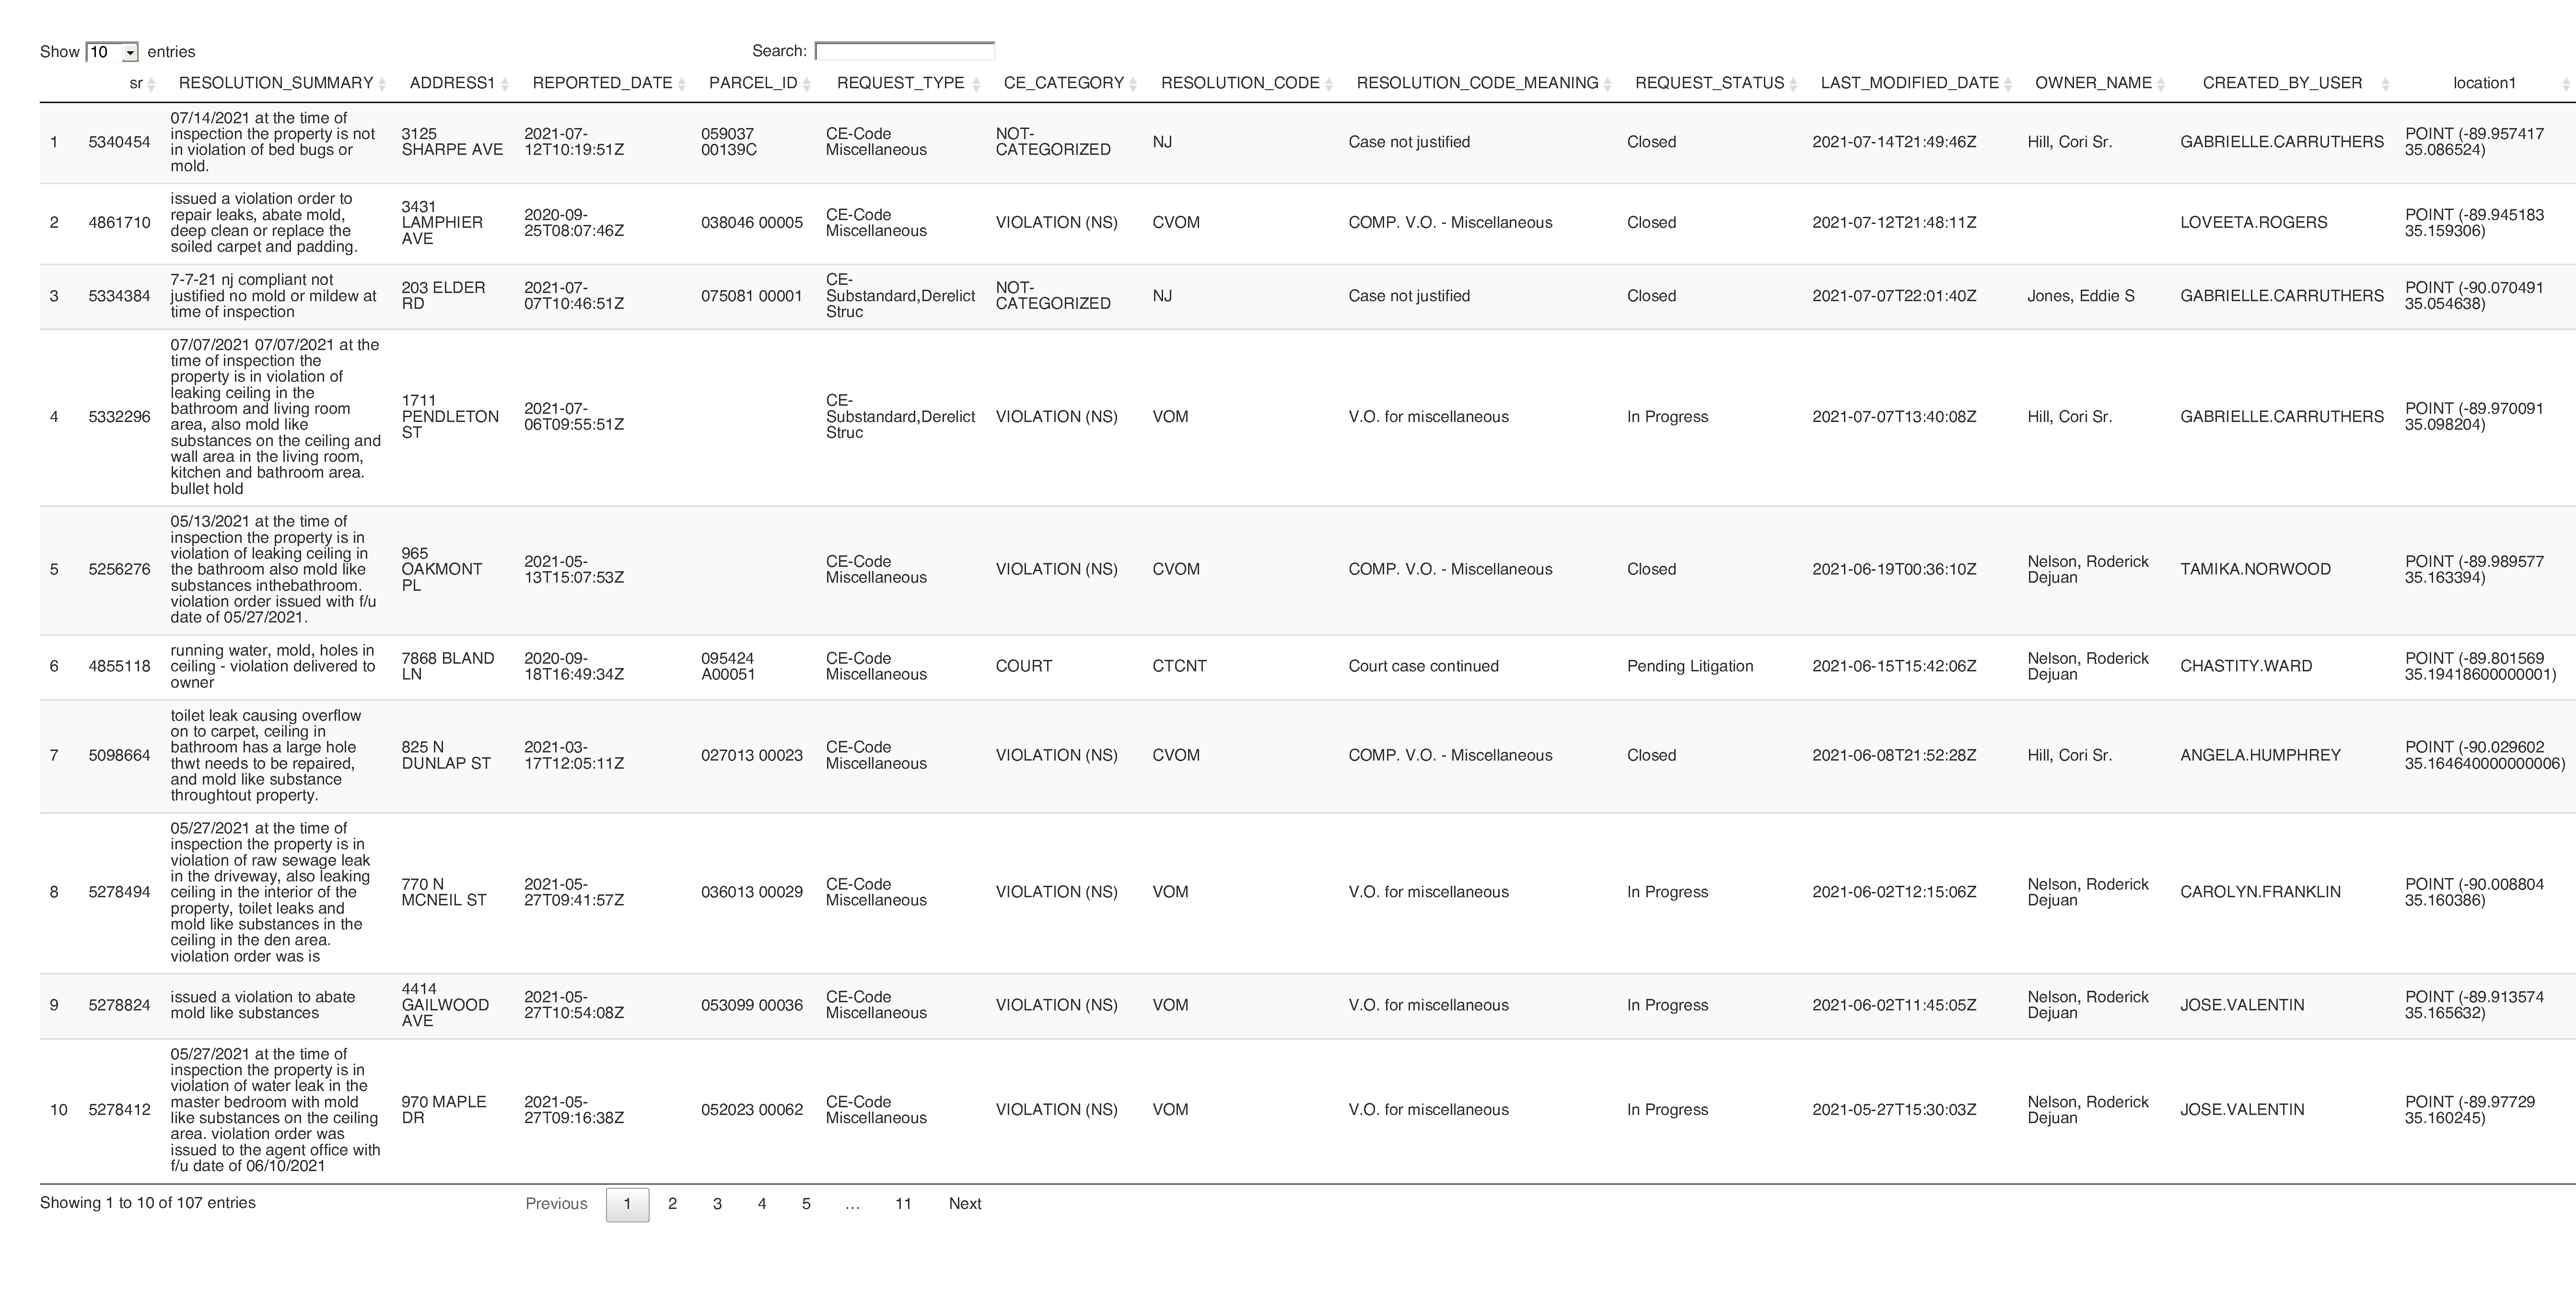
\includegraphics{MA-capstone_files/figure-latex/unnamed-chunk-16-1.pdf}

This search showed that many cases involving tenants do not mention the word tenant. Sometimes ``occupant'' or ``resident'' is used. Other times they are never mentioned; the summary may state a notice was sent to the owner, or make no mention of people at all. This makes it very hard to find information specifically about rental units.

\hypertarget{seeclickfix}{%
\section{SeeClickFix}\label{seeclickfix}}

Another way to view service requests is through Memphis's \href{https://seeclickfix.com/web_portal/DaM5B2x33WeFNJ1zpUeDRvCB/issues/map?lat=35.14896833842707\&lng=-90.05163922905923\&max_lat=35.15402992416014\&max_lng=-90.04691720008852\&min_lat=35.143906437842766\&min_lng=-90.05635857582094\&zoom=17}{SeeClickFix} website. Below we can see how 311 handled a \href{https://seeclickfix.com/web_portal/DaM5B2x33WeFNJ1zpUeDRvCB/issues/10508076}{service request} from a tenant who has been without air conditioning since May.

\begin{longtable}[]{@{}ll@{}}
\toprule
& \\
\midrule
\endhead
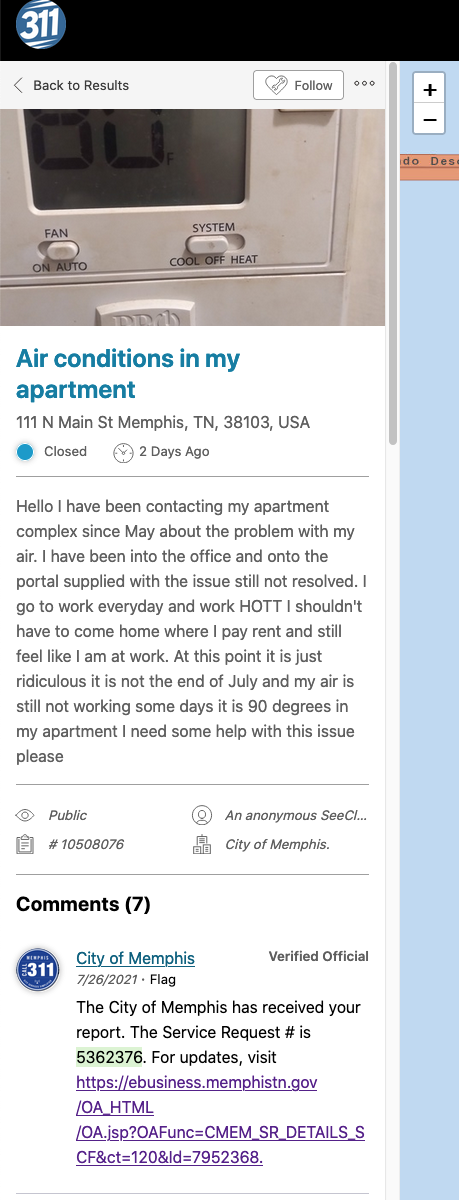
\includegraphics{_img/ACreq1.png} & 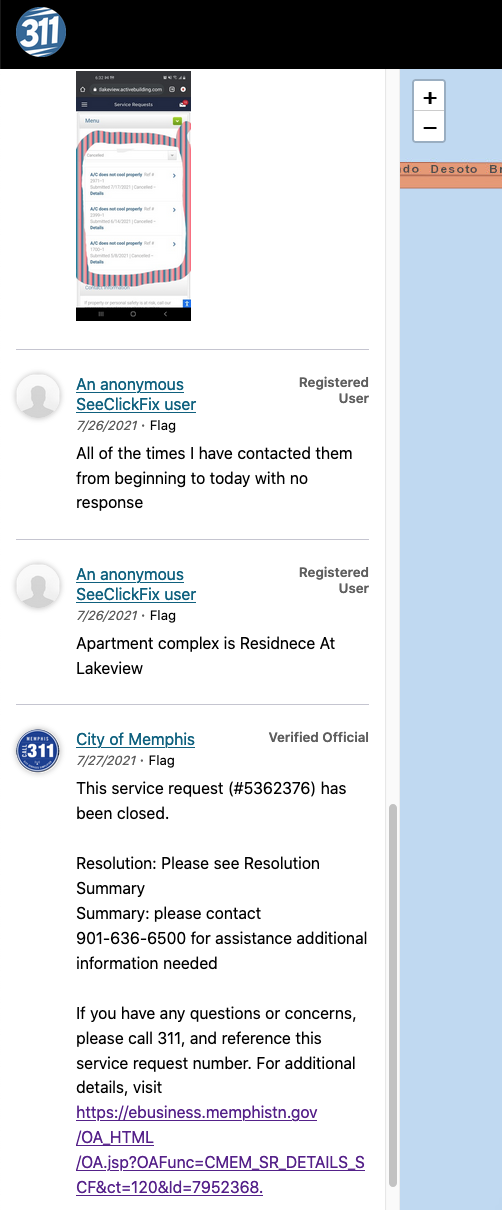
\includegraphics[width=5.1875in,height=\textheight]{_img/ACreq2.png} \\
\bottomrule
\end{longtable}

The tenant provided multiple photos (not all shown here) proving attempts to contact maintenance, which had been canceled or marked as completed though they were not resolved.

\begin{longtable}[]{@{}ll@{}}
\toprule
& \\
\midrule
\endhead
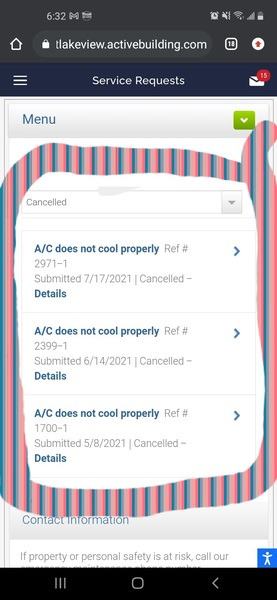
\includegraphics{_img/ACreq3.jpg} & 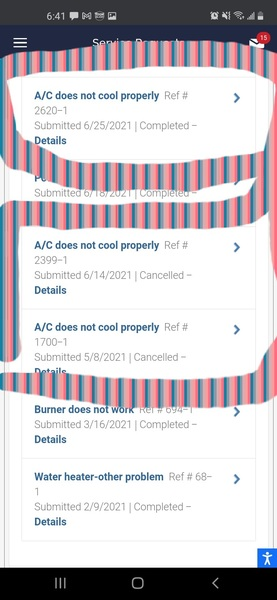
\includegraphics{_img/ACreq5.jpg} \\
\bottomrule
\end{longtable}

Almost immediately, the city closed the request, redirecting the tenant to call a phone number for the Mayor's Citizen Service Center. According to the \href{https://www.memphistn.gov/government/mayor-jim-strickland/mayors-citizen-service-center-311/}{City of Memphis's website}, \textbf{the Mayor's Citizen Service Center is 311}. So it appears 311 closed the request, telling the tenant to contact 311.

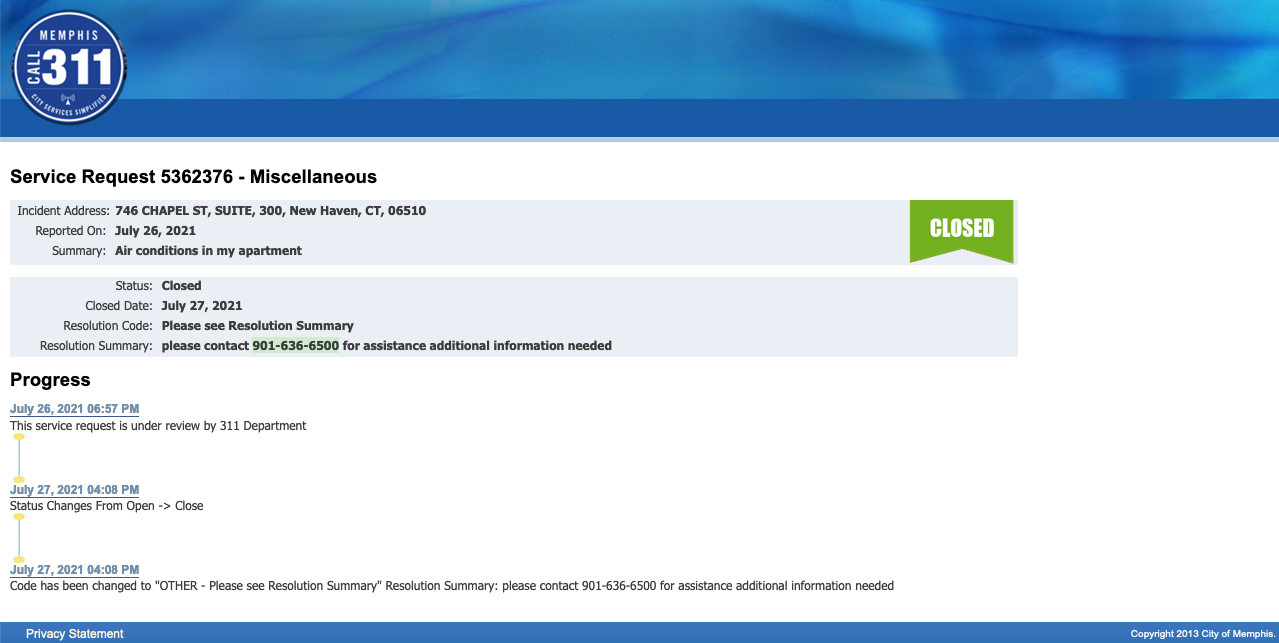
\includegraphics{_img/ACreq4.png}

This was also a case where the incident address was filled in as the 746 Chapel Street, mentioned above as having the most service requests of any address. We can now see the default address is actually in Connecticut.

Unfortunately, this request only revealed additional hurdles in interacting with code enforcement data.

\hypertarget{discussion}{%
\chapter{Discussion}\label{discussion}}

Code enforcement is the only recourse for renters who want to report landlord neglect. However, Memphis code enforcement does not categorize or track this data. Instead, this information is shuffled into a miscellaneous category, with duplicates and errors. While the dataset may be updated daily, it is incredibly hard to organize, and the volume of cases added daily only made the job more difficult.

In conversations with other housing researchers, I found I was not alone in my frustrations with this dataset. I have yet to meet someone who established a way to sort through all the data. One researcher who did regularly use the data did so by limiting the scope/analysis to individual neighborhoods.

This leads me to believe that Memphis code enforcement does not regularly sort through existing data to find trends and patterns. This would not be surprising, except for the department having two lengthy reports over 20 years calling for a strategic, rather than a reactive, code enforcement. A strategic code enforcement requires regular analysis of existing data, to find trends and identify blind spots. Without a strategy, code enforcement will opt for the reactive system. This leads inspectors to spend a disproportionate amount of time on minor violations instead of ones that impact public health. As stated by \protect\hyperlink{ref-betts2001}{Betts},\footnote{\protect\hyperlink{ref-betts2001}{{``Best Practice Number Ten''}}.} ``individual efforts, no matter how well intentioned, are by definition \emph{not strategic}.'' {[}44{]}

Attempting to organize this dataset reminded me of Matthew Desmond discussing the difficulty in finding accurate eviction data for any city just a decade ago. The data existed but it was unorganized and messy. He established the Eviction Lab to draw attention to the problem and help other people access the data. Making the data widely available allowed it to be studied and discussed. The extent of the eviction crisis became apparent, and soon evictions became one of the most important topics in housing.

Public housing in America ended due to mismanagement and neglect of maintenance, and yet few people are calling for the end of private rental housing due to the same practices. Perhaps part of the reason public housing ended was the relative ease of monitoring and tracking the neglect. Information on public housing is publicly available; with relative ease I can find a list of what properties are managed by the city, view the agency plan and yearly financial audit which breaks down revenues and expenses. Meanwhile, trying to find such information about the private rental market is nearly impossible. How are we to hold the private rental market accountable if we don't know the extent of the problem?

\hypertarget{recommendations}{%
\section{Recommendations}\label{recommendations}}

While I recognize that asking an organization to alter its data entry methods is a big ask, I have a few specific recommendations which I believe could completely alter the nature of 311 data.

\begin{enumerate}
\def\labelenumi{\arabic{enumi}.}
\tightlist
\item
  Create a new \texttt{REQUEST\_TYPE} for requests related to private rental/landlord neglect. This would replace at least some of the ``Code Miscellaneous'' category with more substantive information. It might also encourage more tenant reporting, as tenants know they're placing their complaint with the right agency.
\item
  Create a \texttt{RESOLUTION\_CODE} for duplicates, replacing ``JA'' and similar. (For instance ``DUPE'' is used by other cities like \href{https://data.cincinnati-oh.gov/Thriving-Neighborhoods/Code-Enforcement/cncm-znd6}{Cincinnati})
\item
  Do not put all information for one case on one row, overwriting old data. Instead, allow each update its own row.
\item
  Close out old cases which are clearly no open anymore.
\item
  Implement the \textbf{HHRS} into the data system. For occupied housing units, categorize hazards using the HHRS.
\end{enumerate}

\hypertarget{summary}{%
\chapter{Summary}\label{summary}}

The link between housing and health has been well established. Modern humans spend a majority of their time indoors, and the condition of their surroundings inevitably impacts their health. While the quality of new housing has improved overtime, oft overlooked is the quality of existing homes and whether homes are being maintained.

This paper highlights the role of tenure can play in maintenance neglect and enforcement. If a homeowner requires housing maintenance, they are able to directly contract and hire someone to repair the problem; for financially strapped individuals, a wide range of subsidies and grants exist geared towards home repair, upgrades, and weatherization. Yet if a tenant experiences a maintenance problem, ensuring repairs are completed is out of their control. They are entirely reliant upon the landlord to follow through with repairs.

Tenants in low-rent homes can be particularly at risk; their homes are likely older and require more maintenance, and lower rents means lower profit margins, incentivizing low-rent landlords to neglect maintenance to preserve profits. Unless a landlord lives on the property, tenants are the ones burdened with experiencing the effects of the neglect, while the landlord is able to ignore and forget the problem while continuing to receive an income.

Tenants who withhold rent in an attempt to force their landlords to complete repairs are also at risk of eviction. If a landlord opts to ignore a problem, tenants are left in a powerless position with an impossible choice: speak up and risk their housing stability or stay silent and suffer the health consequences of the problem.

Tenants experiencing neglect are incentivized to move to a home with a more responsible owner, or to purchase a home and exit the rental market altogether. This leaves the problem open for future tenants of the home. But increasingly there is not an option for a home that is available, affordable, and in better condition. If a home is affordable and in better condition, the demand will be high and it likely won't be available. If a home is available and in better condition, it is likely more expensive. If a home is available and affordable, the tenant will likely run into the same maintenance issues as their previous home.

The number of people experiencing this dilemma has increased, particularly over the past decade. As a fallout of the Great Recession, many homeowners became renters and homes formerly occupied by owners were converted into rentals. As rent increases have outpaced incomes over the past decade, renters are more likely to be cost burdened than owners, and rents increasingly eat into their ability to save for a down payment. Households can become trapped in rentership, whether they want to rent or not.

While this paper was originally intended to analyze 311 data, it made more apparent the messiness of the dataset and barriers to processing. Hopefully this can lead to collaborative analysis.

\hypertarget{appendix-covid-evictions}{%
\chapter{Appendix: COVID \& Evictions}\label{appendix-covid-evictions}}

\hypertarget{cdc-eviction-moratorium}{%
\section{CDC Eviction Moratorium}\label{cdc-eviction-moratorium}}

When COVID-19 struck, health professionals around the world ordered everyone to stay at home. However, sudden, widespread illness and job loss threatened to displace of millions of Americans who fell behind on rent. The CDC recognized that large waves of evictions could increase the spread of COVID, as people lost a stable place to quarantine and were more likely to double up with family or overcrowd homeless shelters.\footnote{\protect\hyperlink{ref-cdc2020a}{Centers for Disease Control and Prevention, {``HHS/CDC Temporary Halt in Residential Evictions to Prevent the Further Spread of Covid-19,''} 2020}.} Not having shelter also increases a person's risk of severe illness from COVID-19. The risk to public health led the CDC to freeze all evictions due to nonpayment of rent, a power that many did not know they possessed.\footnote{\emph{You're telling me we could've just told them to stop evicting people this whole time??}}

The federal eviction moratorium is set to expire on Saturday, July 31, 2021, the same day this paper will be submitted. Six million families are still behind on rent.\footnote{\protect\hyperlink{ref-sgaier2021}{Sema K. Sgaier and Aaron Dibner-Dunlap, {``They Survived Covid. Now They Face Eviction.''} \emph{The New York Times}, July 28, 2021, \url{https://www.nytimes.com/2021/07/28/opinion/covid-eviction-moratorium.html}}.} The COVID-19 Delta variant, more contagious than smallpox,\footnote{\protect\hyperlink{ref-anthes2021}{Emily Anthes, {``The Delta Variant: What Scientists Know,''} \emph{The New York Times}, June 22, 2021, \url{https://www.nytimes.com/2021/06/22/health/delta-variant-covid.html}}.} has caused a rapid uptick in cases across the U.S. Vaccines have proven effective against severe cases---unvaccinated people account for 97\% of hospitalizations nationwide---\footnote{\protect\hyperlink{ref-mandavilli2021}{Apoorva Mandavilli, {``Vaccinated People May Spread the Virus, Though Rarely, c.d.c. Reports,''} \emph{The New York Times}, July 30, 2021, \url{https://www.nytimes.com/2021/07/30/health/cdc-vaccinated-delta.html}}.}but 40\% of U.S. adults have yet to be fully vaccinated.\footnote{\protect\hyperlink{ref-thenewyorktimes2020}{The New York Times, {``Coronavirus in the u.s.: Latest Map and Case Count,''} \emph{The New York Times}, March 3, 2020, \url{https://www.nytimes.com/interactive/2021/us/covid-cases.html}}.}

The extent of eviction filings and renters in arrears is especially concerning, considering nearly \$50 billion in Emergency Rental Assistance funds has been made available by the federal government.\footnote{\protect\hyperlink{ref-u.s.treasury2021}{U.S. Treasury, {``Emergency Rental Assistance Program,''} July 24, 2021, \url{https://home.treasury.gov/policy-issues/coronavirus/assistance-for-state-local-and-tribal-governments/emergency-rental-assistance-program}}.} Yet stringent requirements, complicated applications, and slow roll-out has meant only a small fraction of renters are getting the assistance they need.\footnote{\protect\hyperlink{ref-deparle2021}{Jason DeParle, {``Federal Aid to Renters Moves Slowly, Leaving Many at Risk,''} \emph{The New York Times}, April 25, 2021, \url{https://www.nytimes.com/2021/04/25/us/politics/rental-assistance-pandemic.html}}.} At the end of June 2021, two states including New York still had not sent out financial assistance to renters.\footnote{\protect\hyperlink{ref-haag2021}{Matthew Haag, {``500,000 New Yorkers Owe Back Rent. What Happens When Evictions Resume?''} \emph{The New York Times}, July 27, 2021, \url{https://www.nytimes.com/2021/07/27/nyregion/evictions-moratorium.html}}.}

\hypertarget{memphis-eviction-settlement-program}{%
\section{Memphis Eviction Settlement Program}\label{memphis-eviction-settlement-program}}

\begin{quote}
Evictions in Memphis are ``a preview of what's to come in the U.S.''

\footnote{\protect\hyperlink{ref-gowen2021}{Annie Gowen, {``She Wanted to Stay. Her Landlord Wanted Her Out.''} \emph{Washington Post}, June 28, 2021, \url{https://www.washingtonpost.com/nation/interactive/2021/eviction-moratorium-lifts/}}.}
\end{quote}

The COVID-19 Delta variant has increased Shelby County's positivity rate from a low of 2.5\% in mid-June to 14.6\% a month later, the highest rate since January.\footnote{\protect\hyperlink{ref-shelbycountyhealthdepartment}{Shelby County Health Department, {``Case Counts: Weekly Test Positivity Rate,''} n.d., \url{https://insight-editor.livestories.com/s/v2/1.2-case-counts/c4f65175-2433-47b7-b112-d62cf719af71}}.} While vaccines have proven effective against severe cases,\footnote{\protect\hyperlink{ref-mandavilli2021}{Mandavilli, {``Vaccinated People May Spread the Virus, Though Rarely, c.d.c. Reports''}}.} only 48\% of all Shelby County adults are fully vaccinated.\footnote{\protect\hyperlink{ref-thenewyorktimes2020}{The New York Times, {``Coronavirus in the u.s.''}}.}\footnote{Age 12+: 45\%; Ages 18+: 48\%; Ages 65+: 69\%.}

As the CDC moratorium ends, an estimated 22\% of all renters in Shelby County are behind in rent.\footnote{\protect\hyperlink{ref-sgaier2021}{Sgaier and Dibner-Dunlap, {``They Survived Covid. Now They Face Eviction.''}}.} However, eviction courts in Memphis have been open since June 15, after a U.S. District Judge sided with landlords who claimed the CDC moratorium overstepped the agency's powers.\footnote{\protect\hyperlink{ref-bailey2021}{Tom Bailey, {``Judge Strikes down Eviction Halt Order,''} \emph{Daily Memphian}, March 16, 2021, \url{https://dailymemphian.com/article/20692/judge-strikes-down-eviction-halt-order-in-memphis}}; \protect\hyperlink{ref-bailey2021a}{Tom Bailey, {``Sixth Circuit Affirms Judge Norris: Eviction Ban Is Not Legal,''} \emph{Daily Memphian}, July 23, 2021, \url{https://dailymemphian.com/article/23083/sixth-circuit-affirms-judge-norris-eviction-ban}}.}

According to Princeton's Eviction Lab, the rate of new filings has increased since the was lifted, though the number of filings remains below historical averages.\footnote{\protect\hyperlink{ref-evictionlab2021}{Eviction Lab, {``Memphis, Tennessee \textbar{} Eviction Tracking System,''} July 31, 2021, \url{https://evictionlab.org/eviction-tracking/memphis-tn/}}.} Compared to 31 other cities nationwide, Memphis ranks 7th in the number of filings during COVID, with 18,166 filings from March 15, 2020 to July 25, 2021.\footnote{To be clear, there was already a housing crisis before Covid. More than 26,000 eviction cases were filed in Shelby County in 2019 alone (\protect\hyperlink{ref-ahmed2021}{Ahmed et al., {``The Effect of State and Local Laws on Evictions,''} 2}).}

Compared to other places, Memphis was able to quickly assist renters and offer relief, though the program was not without faults.

The \textbf{Eviction Settlement Program} (\textbf{ESP}) was established in fall of 2020 with \$2.25 million in funding.\footnote{The following information related to the Eviction Settlement Program was collected from multiple Zoom interviews and meetings with Cindy Ettingoff, chief executive officer of Memphis Area Legal Services, in February and March 2021.} To serve as many people as possible, \textbf{Memphis Area Legal Services} (\textbf{MALS}) offered large lump settlements to landlords who owned complexes where dozens of people have fallen behind on rent. Initially, some landlords refused the offer.

``I had a hard time wrapping my mind around this,'' said Cindy Ettingoff, chief executive officer of MALS, ``but it is true, particularly initially (pre-COVID), that landlords built into the cost of doing business the cost of flipping tenants, going to court, and filing fees, so initially it wasn't as big of a deal to them because that was just part of doing business. They could get someone out and get someone else in.''

Ettingoff emphasized that she is not anti-landlord, and is particularly sympathetic to small landlords, such as those who purchased a duplex or quadplex with retirement money. The goal for the ESP has been to benefit both landlords and tenants.

The bleek outlook of winter 2020 caused landlords to reconsider and accept the offer. By December, the fund was depleted after assisting 1,220 households, with another 1,000 cases which could have been settled with extra funding. The ESP received an additional \$28.2 million in funding in March 2021, and expanded their program to include utility assistance.

The ESP has dispersed over \$10 million of the \$28 million in federal assistance. Yet as the moratorium ends and the economy recovers, landlords may opt to return to the tenant flipping model rather than settle with the existing tenant, as highlighted in a recent Washington Post feature on evictions in Memphis.\footnote{\protect\hyperlink{ref-gowen2021}{Gowen, {``She Wanted to Stay. Her Landlord Wanted Her Out.''}}.} The story centered around a family who had fallen behind on rent in September, was served an eviction notice, received \$1,500 in rental assistance in December and got caught up, only for the landlord to continue with eviction proceedings in June.

As part of the ESP, landlords must agree to not evict a tenant for the months paid for through the program; yet they may evict once the period is over. Tennessee allows landlords large leeway in serving evictions notices; if a tenant's yearly lease has expired, a landlord does not need a cause, only 30-days notice that the tenant has to move out (see \href{http://law.justia.com/codes/tennessee/2010/title-66/chapter-28/part-5/66-28-512}{Tenn. Code Ann. § 66-28-512}). Even if tenants are current on rent, a landlord can order a tenant out by the end of the month.

\begin{figure}
\centering
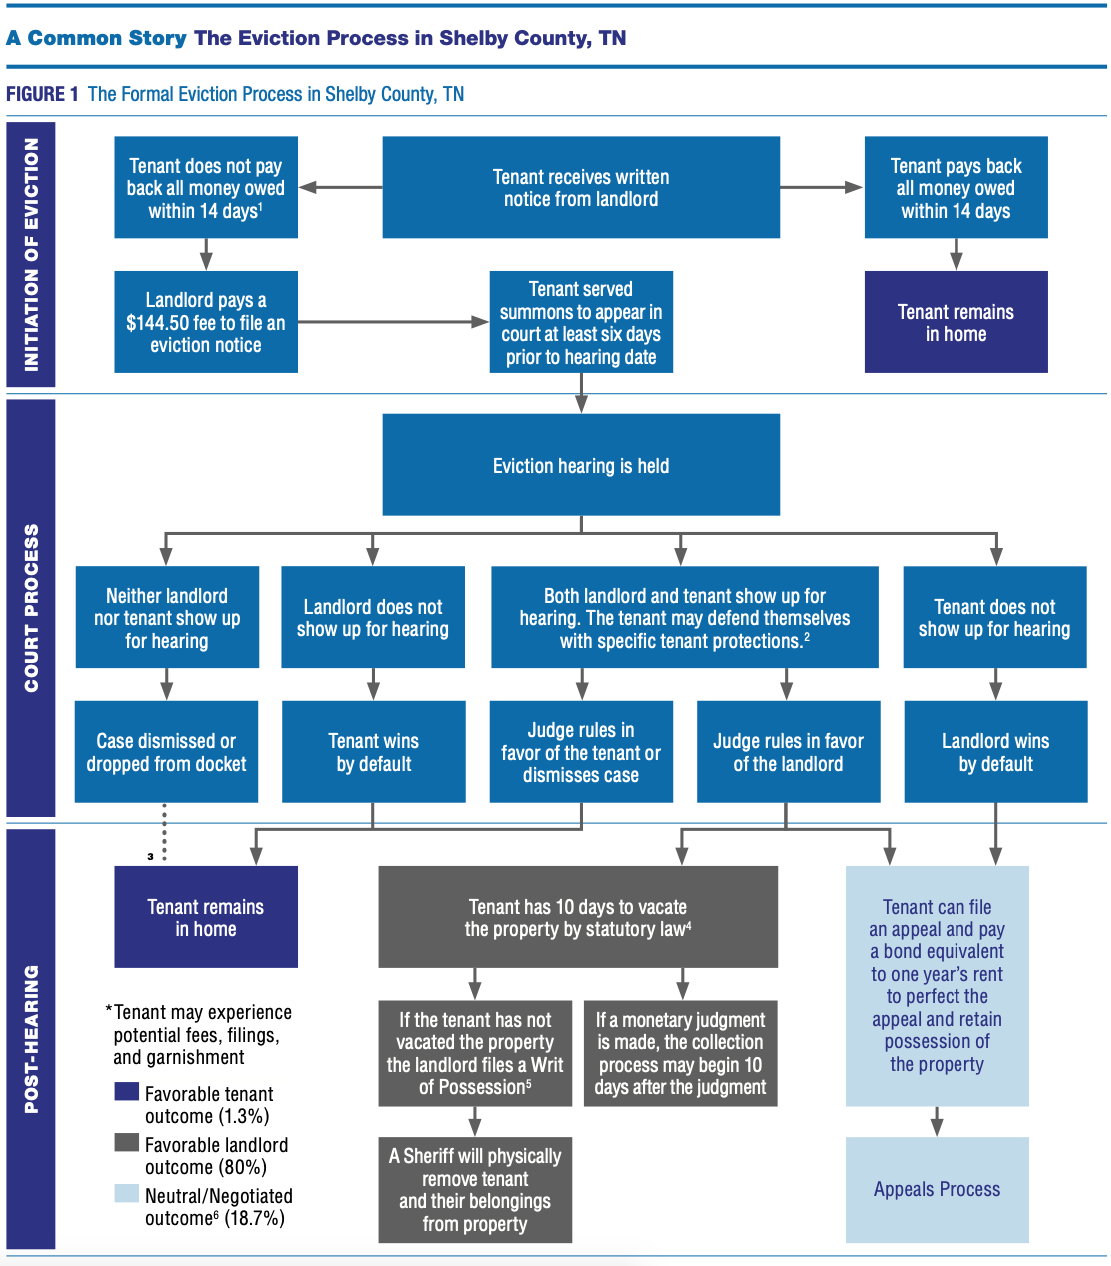
\includegraphics{_img/LSC-shelby-evict.png}
\caption{Source: \href{https://www.lsc.gov/press-release/new-nationwide-lsc-eviction-study-examines-variations-local-laws-and-highlights}{Legal Services Corporation} (2021)}
\end{figure}

If the tenant has not moved after 30 days, they can be served with a summons to appear in court for an eviction hearing. Legal Services Corporation conducted a yearlong study of eviction outcomes in Shelby County for FY 2020 and found 80\% of cases resulted in a favorable landlord outcome, 18.7\% in a neutral or negotiated outcome, and only \textbf{1.3\%} \textbf{end in a favorable tenant outcome}, where the tenant is allowed to remain in the home.\footnote{\protect\hyperlink{ref-ahmed2021}{Ahmed et al., {``The Effect of State and Local Laws on Evictions''}}.}

June 29, 2021, the day after the Washington Post article ran, a volunteer with Memphis Tenants Union called three tenants who had reached out to the group's rental assistance hotline.\footnote{The volunteer allowed me to silently listen in while the calls were taking place.} Of the two tenents who answered, both had the same problem. Each had applied for the ESP and been approved, yet their landlord had denied the settlement and continued with eviction proceedings.

Shelby County's Eviction Settlement Program thrived when the CDC moratorium kept tenants in place and massive layoffs caused high unemployment, giving landlords no immediate chance of income other than accepting the settlement. Now that the moratorium has been lifted and the economy is improving, more landlords may opt to deny funding and resume evictions. This is a problem as the ESP is only structured to distribute rental assistance to landlords, not tenants. This structure can create a scenario where there is a large need for rental assistance from tenants, and a large pool of public funds earmarked for rent relief, but the structure prevents the funds from ever reaching the tenants.

The ESP is allowed to distribute assistance until funding expires in September 2022. Though landlords might deny the funds, relief can also be spent towards utility assistance. As Memphis has a public utility company, there is a slim-to-none chance this relief would be denied.

Still, this outcome begs the question: what was the primary purpose of the rent relief? To keep renters in their home if they lost income due to COVID, or to guarantee landlords the lost income? Ultimately, the program only guaranteed landlords could get paid, not that tenants could keep their housing.

\hypertarget{refs}{}
\begin{CSLReferences}{1}{0}
\leavevmode\hypertarget{ref-aafa2015}{}%
AAFA. {``Asthma Capitals 2015,''} 2015. \url{https://www.aafa.org/media/1607/asthma-capitals-report-2015-rankings.pdf}.

\leavevmode\hypertarget{ref-aafa2021}{}%
---------. {``Asthma Capitals 2021: The Most Challenging Places to Live in with Asthma,''} 2021. \url{https://www.aafa.org/media/3040/aafa-2021-asthma-capitals-report.pdf}.

\leavevmode\hypertarget{ref-ahmed2021}{}%
Ahmed, Ranya, Sarah Abdelhadi, Madeline Youngren, and Carlos Manjarrez. {``The Effect of State and Local Laws on Evictions: The Eviction Process in Shelby County, TN,''} January 2021.

\leavevmode\hypertarget{ref-anthes2021}{}%
Anthes, Emily. {``The Delta Variant: What Scientists Know.''} \emph{The New York Times}, June 22, 2021. \url{https://www.nytimes.com/2021/06/22/health/delta-variant-covid.html}.

\leavevmode\hypertarget{ref-apha1938}{}%
APHA. {``Basic Principles of Healthful Housing.''} \emph{American Journal of Public Health and the Nations Health} 28, no. 3 (March 1938): 351--72. doi:\href{https://doi.org/10.2105/AJPH.28.3.351}{10.2105/AJPH.28.3.351}.

\leavevmode\hypertarget{ref-bailey2021}{}%
Bailey, Tom. {``Judge Strikes down Eviction Halt Order.''} \emph{Daily Memphian}, March 16, 2021. \url{https://dailymemphian.com/article/20692/judge-strikes-down-eviction-halt-order-in-memphis}.

\leavevmode\hypertarget{ref-bailey2021a}{}%
---------. {``Sixth Circuit Affirms Judge Norris: Eviction Ban Is Not Legal.''} \emph{Daily Memphian}, July 23, 2021. \url{https://dailymemphian.com/article/23083/sixth-circuit-affirms-judge-norris-eviction-ban}.

\leavevmode\hypertarget{ref-baker2018}{}%
Baker, Jackson. {``The First 1000 Days of Jim Strickland.''} \emph{Memphis Magazine}, September 3, 2018. \url{https://memphismagazine.com/api/content/65e8dd62-aae1-11e8-9153-120e7ad5cf50/}.

\leavevmode\hypertarget{ref-betts2001}{}%
Betts, Phyllis. {``Best Practice Number Ten: Fixing Broken Windows {{}} Strategies to Strengthen Housing Code Enforcement and Related Approaches to Community-Based Crime Prevention in Memphis,''} April 2001. \url{https://www.pdffiller.com/20879259-BestPracticeNumber10Fixing_Broken_Windowspdf-Best-Practice-Number-Ten-Center-For-Community-Building-and-cbana-memphis-}.

\leavevmode\hypertarget{ref-bradley2019}{}%
Bradley, Cole. {``Seeing Red I: Mapping 90 Years of Redlining in Memphis,''} March 31, 2019. \url{https://www.highgroundnews.com/features/SeeingRedlining.aspx}.

\leavevmode\hypertarget{ref-cdc2020}{}%
CDC. {``Lead in Paint,''} November 24, 2020. \url{https://www.cdc.gov/nceh/lead/prevention/sources/paint.htm}.

\leavevmode\hypertarget{ref-cdc2006}{}%
CDC, and HUD. {``Healthy Housing Reference Manual.''} Atlanta, 2006. \url{https://www.cdc.gov/nceh/publications/books/housing/housing.htm}.

\leavevmode\hypertarget{ref-cdc2020a}{}%
Centers for Disease Control and Prevention. {``HHS/CDC Temporary Halt in Residential Evictions to Prevent the Further Spread of Covid-19,''} 2020.

\leavevmode\hypertarget{ref-chisholm2018}{}%
Chisholm, Elinor, Philipa Howden-Chapman, and Geoff Fougere. {``Tenants{'} Responses to Substandard Housing: Hidden and Invisible Power and the Failure of Rental Housing Regulation.''} \emph{Housing, Theory and Society} 37, no. 2 (October 12, 2018): 139--61. doi:\href{https://doi.org/10.1080/14036096.2018.1538019}{10.1080/14036096.2018.1538019}.

\leavevmode\hypertarget{ref-deparle2021}{}%
DeParle, Jason. {``Federal Aid to Renters Moves Slowly, Leaving Many at Risk.''} \emph{The New York Times}, April 25, 2021. \url{https://www.nytimes.com/2021/04/25/us/politics/rental-assistance-pandemic.html}.

\leavevmode\hypertarget{ref-emergenc1932}{}%
{``Emergency Relief and Construction Act of 1932,''} July 21, 1932. \url{https://uslaw.link/citation/us-law/public/72/302}.

\leavevmode\hypertarget{ref-evictionlab2021}{}%
Eviction Lab. {``Memphis, Tennessee \textbar{} Eviction Tracking System,''} July 31, 2021. \url{https://evictionlab.org/eviction-tracking/memphis-tn/}.

\leavevmode\hypertarget{ref-federalhousingadministration1938}{}%
Federal Housing Administration. {``Underwriting Manual: Underwriting and Valuation Procedure Under Title II of the National Housing Act,''} February 1938. \url{https://www.huduser.gov/portal/publications/Federal-Housing-Administration-Underwriting-Manual.html}.

\leavevmode\hypertarget{ref-goetz2013}{}%
Goetz, Edward G. \emph{New Deal Ruins: Race, Economic Justice, and Public Housing Policy}. Ithaca: Cornell University Press, 2013.

\leavevmode\hypertarget{ref-gowen2021}{}%
Gowen, Annie. {``She Wanted to Stay. Her Landlord Wanted Her Out.''} \emph{Washington Post}, June 28, 2021. \url{https://www.washingtonpost.com/nation/interactive/2021/eviction-moratorium-lifts/}.

\leavevmode\hypertarget{ref-grineski2010}{}%
Grineski, Sara E., and Alma Angelica Hernández. {``Landlords, Fear, and Children's Respiratory Health: An Untold Story of Environmental Injustice in the Central City.''} \emph{Local Environment} 15, no. 3 (March 1, 2010): 199--216. doi:\href{https://doi.org/10.1080/13549830903575562}{10.1080/13549830903575562}.

\leavevmode\hypertarget{ref-haag2021}{}%
Haag, Matthew. {``500,000 New Yorkers Owe Back Rent. What Happens When Evictions Resume?''} \emph{The New York Times}, July 27, 2021. \url{https://www.nytimes.com/2021/07/27/nyregion/evictions-moratorium.html}.

\leavevmode\hypertarget{ref-HHRSover}{}%
HUD. {``Overview of the Healthy Home Rating System,''} n.d. \url{https://www.hud.gov/sites/documents/OVERVIEW_HHRS.PDF}.

\leavevmode\hypertarget{ref-HHRSlst}{}%
---------. {``The Effect of the Defect: Housing Hazards Identified in the Healthy Home Rating System,''} n.d. \url{https://www.hud.gov/sites/documents/hhrschart.pdf}.

\leavevmode\hypertarget{ref-lane2016a}{}%
Lane, Ben. {``BancorpSouth Fined {\$}10.6 Million for Discriminatory Lending, Redlining,''} June 29, 2016. \url{https://www.housingwire.com/articles/37405-bancorpsouth-fined-106-million-for-discriminatory-lending-redlining/}.

\leavevmode\hypertarget{ref-lane2016}{}%
---------. {``First Tennessee Bank Reaches {\$}1.9 Million Settlement over Discriminatory Lending,''} February 1, 2016. \url{https://www.housingwire.com/articles/36175-first-tennessee-bank-reaches-19-million-settlement-over-discriminatory-lending/}.

\leavevmode\hypertarget{ref-lectures1852}{}%
{``Lectures for the People; the Importance of Proper Vetilation.''} \emph{The New York Times}, January 21, 1852. \url{https://www.nytimes.com/1852/01/21/archives/lectures-for-the-people-the-importance-of-proper-vetilation-a.html}.

\leavevmode\hypertarget{ref-mandavilli2021}{}%
Mandavilli, Apoorva. {``Vaccinated People May Spread the Virus, Though Rarely, c.d.c. Reports.''} \emph{The New York Times}, July 30, 2021. \url{https://www.nytimes.com/2021/07/30/health/cdc-vaccinated-delta.html}.

\leavevmode\hypertarget{ref-mccarty2019}{}%
McCarty, Maggie, Libby Perl, and Katie Jones. {``Overview of Federal Housing Assistance Programs and Policy,''} March 27, 2019.

\leavevmode\hypertarget{ref-mclaine2006}{}%
McLaine, Pat, Wendy Shields, Mark Farfel, J. Julian Chisolm, and Sherry Dixon. {``A Coordinated Relocation Strategy for Enhancing Case Management of Lead Poisoned Children: Outcomes and Costs.''} \emph{Journal of Urban Health} 83, no. 1 (January 1, 2006): 111--28. doi:\href{https://doi.org/10.1007/s11524-005-9011-8}{10.1007/s11524-005-9011-8}.

\leavevmode\hypertarget{ref-memphis30}{}%
{``Memphis Comprehensive Planning,''} n.d. \url{https://www.memphis3point0.com}.

\leavevmode\hypertarget{ref-mendell2011}{}%
Mendell, Mark J., Anna G. Mirer, Kerry Cheung, My Tong, and Jeroen Douwes. {``Respiratory and Allergic Health Effects of Dampness, Mold, and Dampness-Related Agents: A Review of the Epidemiologic Evidence.''} \emph{Environmental Health Perspectives} 119, no. 6 (June 1, 2011): 748--56. doi:\href{https://doi.org/10.1289/ehp.1002410}{10.1289/ehp.1002410}.

\leavevmode\hypertarget{ref-federal1985}{}%
Mitchell, J. Paul, Lawrence M. Friedman, and Rutgers University, eds. \emph{Federal Housing Policy and Programs: Past and Present}. New Brunswick, N.J: Center for Urban Policy Research, Rutgers University, 1985.

\leavevmode\hypertarget{ref-national1937}{}%
{``National Housing Act of 1937,''} September 1, 1937.

\leavevmode\hypertarget{ref-national1933}{}%
{``National Industrial Recovery Act of 1933,''} June 16, 1933.

\leavevmode\hypertarget{ref-nelson}{}%
Nelson, Robert K., LaDale Winling, Richard Marciano, Nathan Connolly, and et al. {``Mapping Inequality,''} n.d. \url{https://dsl.richmond.edu/panorama/redlining/}.

\leavevmode\hypertarget{ref-poe2021}{}%
Poe, Ryan. {``Richard Janikowski, 'Father' of Memphis' Blue CRUSH Model of Policing, Dies at 69.''} \emph{The Commercial Appeal}, March 24, 2021. \url{https://www.commercialappeal.com/story/news/local/2021/03/24/richard-janikowski-father-memphis-blue-crush-model-policing-dies-age-69/6966107002/}.

\leavevmode\hypertarget{ref-radford1996}{}%
Radford, Gail. \emph{Modern Housing for America}, 1996. \url{https://press.uchicago.edu/ucp/books/book/chicago/M/bo3636758.html}.

\leavevmode\hypertarget{ref-rauh2002}{}%
Rauh, Virginia A, Ginger R Chew, and Robin S Garfinkel. {``Deteriorated Housing Contributes to High Cockroach Allergen Levels in Inner-City Households.''} \emph{Environmental Health Perspectives} 110, no. suppl 2 (April 1, 2002): 323--27. doi:\href{https://doi.org/10.1289/ehp.02110s2323}{10.1289/ehp.02110s2323}.

\leavevmode\hypertarget{ref-rothacker2012}{}%
Rothacker, Rick. {``Wells Fargo Spending {\$}432 Million to End Lending Suit.''} \emph{Reuters}, May 30, 2012. \url{https://www.reuters.com/article/us-wellsfargo-settlement-idUSBRE84S1H620120530}.

\leavevmode\hypertarget{ref-rothstein2017}{}%
Rothstein, Richard. \emph{The Color of Law: A Forgotten History of How Our Government Segregated America}. First edition. New York London: Liveright Publishing Corporation, a division of W. W. Norton; Company, 2017.

\leavevmode\hypertarget{ref-sellner2021}{}%
Sellner, Michael, and Jordan Wicht. {``How Many American Homes Have Pests?''} April 21, 2021. \url{https://www.census.gov/library/stories/2021/04/how-many-american-homes-have-pests.html}.

\leavevmode\hypertarget{ref-sgaier2021}{}%
Sgaier, Sema K., and Aaron Dibner-Dunlap. {``They Survived Covid. Now They Face Eviction.''} \emph{The New York Times}, July 28, 2021. \url{https://www.nytimes.com/2021/07/28/opinion/covid-eviction-moratorium.html}.

\leavevmode\hypertarget{ref-shelbycountyhealthdepartment}{}%
Shelby County Health Department. {``Case Counts: Weekly Test Positivity Rate,''} n.d. \url{https://insight-editor.livestories.com/s/v2/1.2-case-counts/c4f65175-2433-47b7-b112-d62cf719af71}.

\leavevmode\hypertarget{ref-shin2018}{}%
Shin, Eun Kyong, and Arash Shaban-Nejad. {``Urban Decay and Pediatric Asthma Prevalence in Memphis, Tennessee: Urban Data Integration for Efficient Population Health Surveillance.''} \emph{IEEE Access} 6 (2018): 46281--89. doi:\href{https://doi.org/10.1109/ACCESS.2018.2866069}{10.1109/ACCESS.2018.2866069}.

\leavevmode\hypertarget{ref-soifer2014}{}%
Soifer, Steven, Joseph McNeely, Cathy Costa, and Nancy Pickering-Bernheim. \emph{Community Economic Development in Social Work}. Columbia University Press, 2014.

\leavevmode\hypertarget{ref-stacy2018}{}%
Stacy, Christina Plerhoples, Joseph Schilling, and Steve Barlow. {``Strategic Housing Code Enforcement and Public Health,''} October 17, 2018. \url{https://www.urban.org/research/publication/strategic-housing-code-enforcement-and-public-health}.

\leavevmode\hypertarget{ref-thebuff1854}{}%
{``The Buffalo Poor-House: Horrible Particulars of Its Condition.''} \emph{The New York Times}, July 24, 1854. \url{https://www.nytimes.com/1854/07/24/archives/the-buffalo-poorhousehorrible-particulars-of-its-condition.html}.

\leavevmode\hypertarget{ref-thenewyorktimes2020}{}%
The New York Times. {``Coronavirus in the u.s.: Latest Map and Case Count.''} \emph{The New York Times}, March 3, 2020. \url{https://www.nytimes.com/interactive/2021/us/covid-cases.html}.

\leavevmode\hypertarget{ref-tsai2020}{}%
Tsai, Jack, Natalie Jones, Dorota Szymkowiak, and Robert A. Rosenheck. {``Longitudinal Study of the Housing and Mental Health Outcomes of Tenants Appearing in Eviction Court.''} \emph{Social Psychiatry and Psychiatric Epidemiology}, September 14, 2020. doi:\href{https://doi.org/10.1007/s00127-020-01953-2}{10.1007/s00127-020-01953-2}.

\leavevmode\hypertarget{ref-u.s.treasury2021}{}%
U.S. Treasury. {``Emergency Rental Assistance Program,''} July 24, 2021. \url{https://home.treasury.gov/policy-issues/coronavirus/assistance-for-state-local-and-tribal-governments/emergency-rental-assistance-program}.

\leavevmode\hypertarget{ref-uhlmann2020}{}%
Uhlmann, Alexander. {``The State of Evictions in Memphis, Tennessee.''} University of Texas, Austin, December 2020.

\leavevmode\hypertarget{ref-wurster2020}{}%
Wurster, Catherine Bauer, and Barbara Penner. \emph{Modern Housing}. Minneapolis: University of Minnesota Press, 2020.

\end{CSLReferences}

\end{document}
